%%%%%%%%%%%%%%%%%%%%%%%%%%%%%%%%%%%%%%%%%%%%%%%%%%%%%%%%%%%%%%%%%%%%%
%% This is a "template" model document for submission to the
%% American Chemical Society (ACS).
%%
%% The guidance here contains information about how you may wish to
%% modify it to match the requirements of various ACS journals. The
%% ACS do *not* typeset accepted articles using LaTeX, so there is
%% no specific class required.
%%
%% This template deliberately does *not* seek to reproduce
%% the layout of the typeset journal: this is explicitly not
%% required by the ACS for LaTeX submissions.
%%
%% Please report any issues with the template at
%% https://github.com/josephwright/acs-template/issues
%%
%% Released under the Creative Commons 0 license
%% https://creativecommons.org/public-domain/cc0/
%% 
%% Copyight (c) 2025 Joseph Wright
%%%%%%%%%%%%%%%%%%%%%%%%%%%%%%%%%%%%%%%%%%%%%%%%%%%%%%%%%%%%%%%%%%%%%
\documentclass[letterpaper]{article}

%%%%%%%%%%%%%%%%%%%%%%%%%%%%%%%%%%%%%%%%%%%%%%%%%%%%%%%%%%%%%%%%%%%%%
%% Font setup - delete if you are using LuaLaTeX
%%%%%%%%%%%%%%%%%%%%%%%%%%%%%%%%%%%%%%%%%%%%%%%%%%%%%%%%%%%%%%%%%%%%%
\usepackage[T1]{fontenc}
\usepackage{ctex}

%%%%%%%%%%%%%%%%%%%%%%%%%%%%%%%%%%%%%%%%%%%%%%%%%%%%%%%%%%%%%%%%%%%%%
%% Adjust the margins and allow for line spacing
%%%%%%%%%%%%%%%%%%%%%%%%%%%%%%%%%%%%%%%%%%%%%%%%%%%%%%%%%%%%%%%%%%%%%
\usepackage{geometry}
\geometry{margin = 1in}
\usepackage{setspace}

%%%%%%%%%%%%%%%%%%%%%%%%%%%%%%%%%%%%%%%%%%%%%%%%%%%%%%%%%%%%%%%%%%%%%
%% Reference support
%%
%% The recommended method for producing the reference section is
%% to use biblatex. If you wish to use a classical BibTeX
%% approach, this is easiest to achieve using the achemso package.
%% In that case, you should remove the biblatex lines.
%%%%%%%%%%%%%%%%%%%%%%%%%%%%%%%%%%%%%%%%%%%%%%%%%%%%%%%%%%%%%%%%%%%%%
% You can adjust the printing of DOI, article title, etc. using
% package options, e.g. "doi = true"; see the biblatex manual for
% details of adjusting the number of authors printed, e.g.
% "maxnames = 15" to print no more than 15 authors.
\usepackage[style = chem-acs]{biblatex}
\addbibresource{references.bib}
% If you are using classical BibTeX, remove the above lines and 
% uncomment:
%\usepackage{achemso}

%%%%%%%%%%%%%%%%%%%%%%%%%%%%%%%%%%%%%%%%%%%%%%%%%%%%%%%%%%%%%%%%%%%%%
%% Graphic inclusion and scheme and chart support
%%%%%%%%%%%%%%%%%%%%%%%%%%%%%%%%%%%%%%%%%%%%%%%%%%%%%%%%%%%%%%%%%%%%%
\usepackage{graphicx}
\usepackage{float}
\usepackage{amsmath,tabularx,placeins}
\setlength{\emergencystretch}{2em}
% 补充表跨页排版及历史稿 Unicode 字符兼容；均使用现有 TeX Live 宏包。
\usepackage{array,longtable,booktabs,newunicodechar}
\newunicodechar{–}{\textendash}
\newunicodechar{—}{\textemdash}
\newunicodechar{‐}{-}
\newunicodechar{ń}{\'{n}}
\newunicodechar{μ}{\ensuremath{\mu}}
\newunicodechar{γ}{\ensuremath{\gamma}}
\newunicodechar{δ}{\ensuremath{\delta}}
\newunicodechar{α}{\ensuremath{\alpha}}

\usepackage{xcolor}
\usepackage{pgfplots}
\pgfplotsset{compat = 1.18}
\definecolor{acsblue}{RGB}{72,116,176}
\definecolor{acsred}{RGB}{196,78,82}
\definecolor{acsorange}{RGB}{221,132,82}
\definecolor{acsgray}{RGB}{88,89,91}
\definecolor{acsplotbg}{RGB}{239,241,247}
\pgfplotsset{
  acs axis/.style={
    axis background/.style={fill=acsplotbg},
    axis line style={draw=acsgray, line width=0.45pt},
    tick style={draw=acsgray, line width=0.4pt},
    tick label style={font=\footnotesize},
    label style={font=\small},
    title style={font=\small\bfseries},
    grid=both,
    major grid style={draw=white, line width=0.55pt},
    minor grid style={draw=white, line width=0.3pt},
    minor tick num=1,
    scaled ticks=false,
    legend style={draw=none, fill=none, font=\footnotesize},
    every axis plot/.append style={line width=0.85pt}
  },
  acs xbar/.style={
    acs axis,
    xbar,
    xmin=0,
    width=0.88\linewidth,
    height=6.1cm,
    bar width=8pt,
    enlarge y limits=0.16,
    nodes near coords,
    nodes near coords align={horizontal},
    nodes near coords style={font=\scriptsize, xshift=1.2pt}
  },
  acs ybar/.style={
    acs axis,
    ybar,
    width=0.92\linewidth,
    height=6.1cm,
    bar width=11pt,
    enlarge x limits=0.08,
    nodes near coords,
    nodes near coords align={vertical},
    nodes near coords style={font=\scriptsize, yshift=1pt}
  }
}
\newfloat{scheme}{htbp}{los}
\floatname{scheme}{Scheme}
\floatname{chart}{Chart}
\newfloat{graph}{htbp}{loh}

%%%%%%%%%%%%%%%%%%%%%%%%%%%%%%%%%%%%%%%%%%%%%%%%%%%%%%%%%%%%%%%%%%%%%
%% Common support packages
%%%%%%%%%%%%%%%%%%%%%%%%%%%%%%%%%%%%%%%%%%%%%%%%%%%%%%%%%%%%%%%%%%%%%
\usepackage{chemformula} % Formulas using \ch{}
% or
\usepackage[version = 4]{mhchem} % Formulas using \ce{}

%%%%%%%%%%%%%%%%%%%%%%%%%%%%%%%%%%%%%%%%%%%%%%%%%%%%%%%%%%%%%%%%%%%%%
%% Many journals require that sections are unnumbered: this 
%% is activated here
%%%%%%%%%%%%%%%%%%%%%%%%%%%%%%%%%%%%%%%%%%%%%%%%%%%%%%%%%%%%%%%%%%%%%
\setcounter{secnumdepth}{-1}

%%%%%%%%%%%%%%%%%%%%%%%%%%%%%%%%%%%%%%%%%%%%%%%%%%%%%%%%%%%%%%%%%%%%%
%% Place any additional macros here.  Please use \newcommand* where
%% possible, and avoid layout-changing macros (which are not used
%% when typesetting).
%%%%%%%%%%%%%%%%%%%%%%%%%%%%%%%%%%%%%%%%%%%%%%%%%%%%%%%%%%%%%%%%%%%%%
\newcommand*\mycommand[1]{\texttt{\emph{#1}}}

%%%%%%%%%%%%%%%%%%%%%%%%%%%%%%%%%%%%%%%%%%%%%%%%%%%%%%%%%%%%%%%%%%%%%
%% Author and title data:
%% the authblk package is currently the simplest way to provide this
%%%%%%%%%%%%%%%%%%%%%%%%%%%%%%%%%%%%%%%%%%%%%%%%%%%%%%%%%%%%%%%%%%%%%
\usepackage{authblk}
\author[1]{Xinge Xia}
\author[1]{Fan Wu}
\affil[1]{College of Cyber Security, Jinan University, Guangzhou, China}
\author[2]{Xianyou Duan}
\affil[2]{College of Chemistry and Materials Science, Jinan University, Guangzhou, China}
\author[1]{Hongyi Chen}
\author[1]{Bingwen Feng}
\author[2]{Ting Liu}

\title{纳米硒细胞毒性预测：从材料化学特征建模到分组验证与 HUVEC 实验评价}
% Use the \date command for email address(s) of corresponding authors
\date{*Email: i.k.groupleader@unknown.uu}

\begin{document}

\maketitle

\begin{abstract}
  针对纳米硒（SeNPs）细胞毒性评价实验成本高、可用检测数据有限的问题，本研究基于已有文献数据和结合其材料理化特性构建了关于SeNPs的细胞存活率预测模型。通过比较多种机器学习方法，我们考察了材料化学特征对细胞毒性预测性能的影响，并采用按文献来源分组的交叉验证验证模型的泛化能力。在收集到的纳米硒数据上进行实验，随机森林基础模型表现最佳，平均绝对误差（MAE）为 19.11。在此基础上，我们进一步对 9 种纳米硒材料开展人脐静脉内皮细胞（HUVEC）实验，在不同浓度和暴露时间条件下获得 351 组预测与实测配对数据，预测 MAE 为 14.51，决定系数（$R^2$）为 0.447。结果表明，该模型能够在一定程度上预测新材料的细胞存活率，在较长暴露时间下的响应变化及在不同材料和作用时间下材料间毒性差异，是进一步提高预测精度的重点。本研究将文献数据建模与新材料实验检验相结合，可为纳米硒细胞毒性预测及材料初步筛选提供参考。

\end{abstract}

\section*{Keywords}

纳米硒；细胞毒性；材料化学特征；文献分组验证；HUVEC；外部预测评价

\section*{Abbreviations}

SeNPs，纳米硒；RF，随机森林；HUVEC，人脐静脉内皮细胞；OOF，折外预测；MAE，平均绝对误差；RMSE，均方根误差；IC50，半数抑制浓度。

%%%%%%%%%%%%%%%%%%%%%%%%%%%%%%%%%%%%%%%%%%%%%%%%%%%%%%%%%%%%%%%%%%%%%
%% Start the main part of the manuscript here.
%%%%%%%%%%%%%%%%%%%%%%%%%%%%%%%%%%%%%%%%%%%%%%%%%%%%%%%%%%%%%%%%%%%%%
\section{引言}

硒是哺乳动物必需的微量元素，参与谷胱甘肽过氧化物酶等硒蛋白的合成，在维持机体氧化还原稳态中发挥重要作用。与亚硒酸盐、硒酸盐等无机硒相比，零价态纳米硒在部分研究中表现出较高的生物利用度和较低的急性毒性，在抗肿瘤、抗菌、抗糖尿病及抗氧化等生物医学领域具有应用潜力\cite{hosnedlova2018nanoselenium,bisht2022senps,sowmya2024nanoselenium,karthik2024senps}。然而，硒的有效剂量与毒性剂量较为接近，纳米化也不能完全消除其毒性风险。研究发现，纳米硒在发挥生物学作用的同时，仍可能引起氧化损伤和细胞毒性\cite{wang2020prooxidation}。过量硒暴露还可能造成消化系统、呼吸系统及心血管系统等损伤\cite{hosnedlova2018nanoselenium}。因此，预测纳米硒在不同材料性质和暴露条件下的毒性，是其生物医学应用的重要基础。

纳米硒的细胞毒性与粒径、暴露浓度、暴露时间及表面修饰等因素密切相关。粒径减小可增加颗粒的比表面积，影响其生物活性和细胞摄取过程，也可能会增加毒性风险\cite{zhang2023senpsbio}。在暴露浓度方面，Wang 等\cite{wang2020prooxidation}发现，大鼠肝细胞暴露于 24~$\mu$M 和 48~$\mu$M 纳米硒 24~h 后，细胞存活率分别降至 87.76\% 和 51.37\%，表现出剂量依赖性。表面修饰也会改变纳米硒与细胞的相互作用。例如，螺旋藻多糖（SPS）、江蓠多糖（GLP）及黄芪多糖（AASP）修饰的纳米硒在相关研究中表现出对肿瘤细胞的选择性杀伤作用，同时对正常细胞的毒性较低\cite{zhang2023senpsbio,ji2023astragalus}；季铵化壳聚糖--没食子酸修饰的纳米硒则在 Colo357 和 HaCaT 细胞中表现出较高的细胞毒性\cite{lunkov2023chitosan}。这些结果说明，不同纳米硒材料的毒性不能仅由单一性质判断，需要结合材料特征、细胞类型和暴露条件进行考虑。

传统纳米毒性评价主要依赖体外细胞实验和体内动物实验，但实验周期、成本及检测通量等因素限制了其在大量材料筛选中的应用\cite{ahmadi2024toxicity}。此外，纳米材料的粒径、形貌、表面性质和化学组成等因素共同影响毒性，其与生物效应之间的关系较为复杂\cite{ji2025rosml}。随着计算毒理学的发展，纳米定量构效关系（nano-QSAR）和定量结构--毒性关系（nano-QSTR）等方法被用于分析材料性质与毒性之间的关系，成为实验评价的补充\cite{roy2023tio2}。其中，随机森林、支持向量机和神经网络等机器学习方法已经被用于金属及金属氧化物纳米颗粒的细胞毒性预测\cite{zhang2023qsar}。另外，为了改善模型的预测表现，研究人员针对机器学习方法结合特征筛选、聚类分析和参数优化进行了进一步的研究\cite{sang2022mlcytotoxicity}。

已有研究展示了机器学习在纳米毒性预测中的应用潜力。Shirokii 等通过相关性特征筛选和网格搜索优化模型参数，构建的无机纳米材料细胞毒性预测模型在 10 折交叉验证中表现良好，$Q^2$ 达到 0.86\cite{shirokii2023quantitative}。Hosni 等的研究表明，LightGBM 在所比较的模型中具有较好的纳米颗粒细胞毒性分类性能\cite{hosni2025mlnp}。此外，Boruta-RF-ARM 组合方法识别了浓度、核壳材料及细胞类型等与毒性相关的重要因素\cite{yildirim2025rheumatoid}。然而，现有模型多面向多种纳米材料，对纳米硒及其表面修饰差异的考虑仍不充分。因此，有必要结合纳米硒的材料性质与暴露条件建立细胞毒性预测模型，为实验前的毒性评估和材料初步筛选提供参考。

基于上述问题，本研究以细胞存活率为预测目标，进行以下研究贡献：
\begin{itemize}
\item[1)]利用通用纳米颗粒和纳米硒文献数据，比较不同机器学习模型的预测性能，结合材料化学特征、特征筛选和多模态信息开展建模;
\item[2)]利按文献来源分组评价模型的泛化能力，考察迁移学习及浓度与暴露时间交互项对预测性能的影响;
\item[3)]利开展 9 种纳米硒材料的人脐静脉内皮细胞（HUVEC）实验，通过预测结果与实测结果的比较，检验模型对新材料细胞存活率及毒性差异的预测能力。
\end{itemize}

本研究旨在探索依据材料性质和暴露条件预测纳米硒细胞毒性的方法，为实验前的毒性评估与材料初步筛选提供参考。

\section{方法}

本研究按数据整理、模型建立和新材料检验的顺序推进。预实验我们从已发表文献中整理纳米硒细胞实验记录，并以论文 \cite{masarkar2024} 中的纳米材料数据作为参照，比较不同模型预测细胞存活率的表现。
在正式实验中，我们基于前期进行的预实验继续补充了文献实验记录和可获得的新的材料表征信息，并比较基础特征与新增特征的作用。
为检验模型对不同文献的预测能力，我们对数据进行了核对并按文献来源分组检验模型性能。
随后我们针对 9 种纳米硒材料开展 人脐静脉内皮细胞(HUVEC) 细胞实验，在不同浓度和暴露时间下测量细胞存活率，并与模型预测的预测结果进行比较。
各步骤所用数据和评价方法在下文分别说明。

\subsection{预实验：文献数据整理、模型比较与特征工程}

\paragraph{数据收集}
%我们首先在通用数据集以及自建数据集上进行模型训练和预测，用于探索模型能否进行细胞毒性的预测以及纳米硒材料特征的是否可用（？，详细的数据集构成如下。
我们首先利用通用纳米材料数据集和自建纳米硒数据集训练并进行模型预测，研究模型预测细胞存活率的能力以及纳米硒材料特征能否为预测提供额外信息。两个数据集的构成如下：
\begin{enumerate}
  \item \textbf{通用数据集：}
该数据集来源于 Masarkar 等人 \cite{masarkar2024} 开展的纳米颗粒细胞毒性元分析研究。
数据集汇总了关于金属、金属氧化物、聚合物以及碳基纳米颗粒四大类别的细胞毒性实验数据，是当前纳米材料机器学习毒性预测领域具有代表性的公开数据资源之一。
本研究的模型改进工作是在其原有框架基础上展开，因此采用该数据集对基线模型进行复现，以保证模型优化过程具备良好的可比性与有效性。
该数据集原始共包含 4111 条实验记录，经清洗后保留 4102 个有效样本用于后续训练测试划分与模型比较。

  \item \textbf{自建数据集：}
针对纳米硒这一特定研究对象，本研究从 43 篇发表于 2008--2022 年的同行评议文献中系统提取实验记录，构建纳米硒细胞毒性预测专项数据集。
数据整理采用大模型粗提取与人工精校验证相结合的流程，详细的是利用提示词工程，引导大模型按照 Masarkar 等人\cite{masarkar2024} 的特征体系提取 43 篇文献中的特征属性；
对于正文未明确报告而可从图表获得的数据，进行人工数字化提取；
最后逐项对照原始文献核验全部记录。
来源文献完整清单见补充材料表~\ref{tab:source-publications}。整理后共包含 383 条有效记录，每条记录对应 37 个特征参数，覆盖纳米硒理化性质、暴露条件及生物学终点，是增强预测模型的训练、验证与评价提供数据基础。
\end{enumerate}

为进一步说明自建数据集的文献来源结构，本研究按题名和研究目的将 43 篇纳米硒相关文献划分为四类：材料构建/表面修饰、机制毒理/安全性、递送/联合治疗、诊疗/免疫及其他应用，该分类仅用于展示文献覆盖范围和主题分布。图~\ref{fig:senp-literature-cloud} 展示文献发表年份与主题分类的点云分布。

\begin{figure}[H]
  \centering
  \begin{tikzpicture}
    \begin{axis}[
      acs axis,
      width=0.82\linewidth,
      height=6.5cm,
      xmin=2007.5,
      xmax=2022.8,
      ymin=0.55,
      ymax=4.45,
      xlabel={发表年份},
      xtick={2008,2010,2012,2014,2016,2018,2020,2022},
      ytick={1,2,3,4},
      yticklabels={材料/表面,机制/安全,递送/联合,诊疗/免疫/其他},
      y tick label style={font=\scriptsize},
      title={\textbf{(A)} 43 篇文献点云}
    ]
      \addplot+[only marks, mark=*, mark size=1.9pt, acsblue] coordinates {
        (2008,0.78) (2011,1.10) (2011.88,0.92) (2012.12,1.24)
        (2012.36,0.80) (2013.16,1.08) (2014,0.92) (2019,1.20)
      };
      \addplot+[only marks, mark=square*, mark size=1.8pt, acsred] coordinates {
        (2011.15,1.80) (2012.86,2.08) (2013.05,1.86)
        (2013.30,2.22) (2018,1.92) (2019.15,2.12)
      };
      \addplot+[only marks, mark=triangle*, mark size=2.1pt, acsorange] coordinates {
        (2012.44,2.76) (2012.68,3.18) (2013.42,2.90) (2014.04,3.24)
        (2014.32,2.78) (2015,3.12) (2015.96,2.86) (2016.22,3.22)
        (2017,2.94) (2018.16,3.16) (2019.30,2.84) (2020,3.12)
        (2021,2.90) (2021.24,3.20)
      };
      \addplot+[only marks, mark=diamond*, mark size=2pt, acsgray] coordinates {
        (2016.34,3.78) (2016.54,4.06) (2016.74,4.30) (2018.30,3.88)
        (2018.50,4.18) (2019.44,3.78) (2019.64,4.08) (2019.84,4.30)
        (2020.14,3.92) (2021.34,4.20) (2021.54,3.84) (2022,4.10)
        (2022.18,3.78) (2022.36,4.30) (2022.54,3.96)
      };
    \end{axis}
  \end{tikzpicture}

  \vspace{0.8em}

  \begin{tikzpicture}
    \begin{axis}[
      acs xbar,
      width=0.62\linewidth,
      height=4.6cm,
      xmax=16,
      xlabel={文献数量},
      symbolic y coords={机制/安全,材料/表面,递送/联合,诊疗/免疫/其他},
      ytick=data,
      y tick label style={font=\scriptsize},
      title={\textbf{(B)} 分类数量}
    ]
      \addplot+[fill=acsblue, draw=none] coordinates {(6,机制/安全) (8,材料/表面) (14,递送/联合) (15,诊疗/免疫/其他)};
    \end{axis}
  \end{tikzpicture}
  \caption{自建纳米硒数据集 43 篇来源文献的发表年份点云与主题分类分布。}
  \label{fig:senp-literature-cloud}
\end{figure}

\paragraph{数据预处理}
对于通用数据集，我们使用 Masarkar 等人 \cite{masarkar2024} 的预处理方案：
首先，删除数据集中包含大量缺失值的特征属性，例如多分散指数 PDI 和长径比，以及与预测无关的文献信息，如文章 ID、发表年份和 DOI 编号，将 30 个特征精简至 15 个有效特征。
其次，对于某些在物理化学性质上存在严重信息确实的纳米颗粒，如缺少尺寸、Zeta 电位、表面电荷以及 PDI，我们剔除了其对应的所有数据点。

随后，我们将剩余的数据集按照材料类型统一划分为四大类纳米颗粒：金属（M）、金属氧化物（MO）、聚合物（P）和碳基（C）纳米颗粒。
在处理具体的物理化学特征时，为了整合不同测试条件下的数据，我们采用了以下优先级策略：

\begin{enumerate}
  \item \textbf{尺寸（Size）特征}：
优先采用无任何介质条件下的尺寸；若该值缺失但提供了水中和培养基中的尺寸，则采用水中的尺寸；若原数据仅提供了一种条件（无介质、水中或培养基中）下的尺寸，则直接使用该已知值。

  \item \textbf{Zeta 电位特征}：
采用类似策略，优先采用水中的 Zeta 电位；若仅提供了一种条件下的 Zeta 电位，则直接使用该值。
\end{enumerate}

在执行上述整合、审查目标变量缺失并严格过滤异常值后，最终清洗后的数据集保留了 4102 个有效数据点和 15 个特征属性。
最后，为了使数据完全适合模型训练，我们使用“min-max”缩放器（MinMaxScaler）对编译后的数据集进行了归一化处理，并对所有的类别属性进行了标签编码（Label encoding）。

对于自建的纳米硒专项数据集，预处理步骤进行了改进。
本研究自建的纳米硒毒性数据集共包含 383 个样本与 37 个特征。
数据集覆盖了纳米硒研究中常见的实验条件区间，包括不同的暴露剂量、粒径范围、形态类型与表面修饰策略，可反映纳米硒与其理化性质的关系在多个维度上的变化。

自建数据集数据预处理包括以下步骤：

\begin{enumerate}
  \item \textbf{缺失值处理}：由于粒径、Zeta 电位、暴露时间、浓度、细胞存活率诸字段都有若干缺失值，故首先直接剔除含缺失值的记录。此外，“检测方法”字段中若干条目“Characterization”“Western”“Cellular Uptake”属于非毒性检测目的条目，故一并删除。最终共剔除 262 条记录，保留 383 个符合要求的有效样本。
  \textbf{上述剔除仅针对所列关键字段；派生特征（如粒径比）和非关键分类变量（如表面电荷）的缺失值在剔除之后单独处理，不在此列。}

  \item \textbf{多报告值的优先级选择}：参照 Masarkar 等人 \cite{masarkar2024} 提出的方法：同一纳米颗粒在文献中报告多种尺寸时，按无介质中的粒径 > 水相粒径 > 培养基中的粒径的顺序选取，而 Zeta 电位宜取水相测量值，若无该数据则取文献中所给的唯一测量值。

  \item \textbf{单位统一与换算}：把各浓度单位都统一换算为 $\mu$g/mL，凡以 $\mu$M 为单位的浓度都根据硒的分子量（78.96 g/mol）换算为 $\mu$g/mL，同时把暴露时间统一转换为小时（h）。

  \item \textbf{数值特征变换}：由于浓度、时间两变量都呈偏态分布，对二者做对数变换：
        \[
          \text{Log\_Conc} = \ln(1 + \text{Concentration\_μg/mL}), \quad
          \text{Log\_Time} = \ln(1 + \text{Time\_h})
        \]
        同时引入“粒径比”= 水合粒径 / 核心粒径来表征颗粒在水相中的聚集倾向，所有缺失值均按 1.5 填充。

  \item \textbf{分类变量编码}：对表面电荷（正/负/中性）、细胞类型、修饰基团、检测方法、晶型（结晶/无定形）等类别特征，采用标签编码转换为数值，其中表面电荷缺失值填充为“未知”。

  \item \textbf{相关性检查}：对数值特征计算 Pearson 相关系数，未发现 $r > 0.8$ 的高相关度特征对，表明特征冗余度很低。
\end{enumerate}

\paragraph{特征工程与多模态融合}

在此基础上，模型输入特征被组织为基础特征和增强特征两组。基础特征包含以下几类信息：暴露条件（浓度、时间）、颗粒理化属性（粒径、Zeta 电位、尺寸比、表面电荷）、生物体系属性（细胞类型）以及实验条件（检测方法、修饰基团）。
针对硒纳米颗粒专用建模，在基础特征之外进一步引入 5 项增强变量，即 IC50、元素 Se 含量、长期稳定性、Se 3d 结合能 和晶型编码。其中，元素 Se 含量、长期稳定性、Se 3d 结合能 与晶型编码主要用于表征材料本征化学属性；IC50 则与毒理响应终点具有较强关联，因此本文将其视为辅助变量，用于比较含/不含该变量时模型表现的差异，而不将其简单等同于可在真实预测前稳定获得的先验理化特征。

为利用不同特征模态之间的互补信息，本研究采用多模态特征融合策略，将输入划分为三个模态：（1）基础理化描述符，包括浓度、时间、粒径、Zeta 电位、尺寸比、表面电荷、细胞类型、检测方法和修饰基团；（2）材料化学增强描述符，包括元素 Se 含量、长期稳定性、Se 3d 结合能和晶型编码；（3）可选辅助描述符 IC50。融合分为三个阶段：首先拼接基础特征与材料化学增强特征，构建联合表示；随后，在 IC50 可用时以其作为查询，对联合表示计算交叉注意力权重，自适应突出相关特征，而在 IC50 缺失时旁路注意力机制、直接使用联合表示；最后加入残差连接以保留原始联合表示，并将所得多模态特征矩阵输入预测模型。该设计将材料本征化学信息与通用理化描述符整合，并根据辅助信息是否可用动态调整特征权重。

为评估新增增强信息对模型性能的提升作用，保持基础特征不变，对上述 5 项增强变量的全部非空组合进行穷举搜索，共 31 种组合，并以三折交叉验证 MAE 作为筛选指标，用于确定表现较优的增强变量子集。需要指出的是，若最优组合包含 IC50，则其结果更适合作为辅助分析依据，而不宜直接等同于真实部署情境下的预测能力提升。

\paragraph{模型与预测}
本研究围绕表格型纳米毒性数据比较了树模型、注意力增强树模型与深度表格模型三类方法。在基准数据集上，纳入随机森林、XGBoost、ABRF、LARF、TabTransformer 和蒸馏 TabTransformer 六种模型，以系统评估不同架构对异质纳米颗粒数据的适应性；在硒纳米颗粒专用数据集上，重点比较基础特征与增强特征条件下各模型的性能差异。随机森林作为核心基线模型，用于评估中小样本场景下的稳健性与可解释性；XGBoost 用于测试梯度提升树在增强特征条件下的高精度建模能力；ABRF 与 LARF 用于考察注意力机制引入后是否能够提升树模型表现；TabTransformer 与蒸馏 TabTransformer 则作为深度表格模型代表，用于与传统树模型进行对照。

本文对模型性能采用回归、分类两类指标进行评价。回归任务中采用决定系数（\(R^2\)）、平均绝对误差（MAE）和均方根误差（RMSE）。\(R^2\) 是对模型所拟合的目标变量方差的解释比例的自然度量，理论上不超过 1（当模型表现差于均值基线时可能为负值），越接近 1 表明拟合效果越好。MAE 是预测值与真实值绝对误差的算术平均，其单位与目标变量一致（\%），因此也是预测典型偏差的直接度量。RMSE 对较大误差更敏感，适用于考察预测的稳定性。

分类任务沿用 Masarkar 等人\cite{masarkar2024} 所采用的 85\% 细胞存活率阈值，将样本划分为“高存活”和“低存活”两类，以保持与基准数据集一致并便于直接比较模型表现，继而用准确率（Accuracy）、F1 分数和 ROC 曲线下面积（AUC）作为主要指标。准确率即正确分类的比例，F1 分数是精确率、召回率的调和平均，对类别不平衡问题具有适应性，而 AUC 衡量模型区分正负类的能力，0.5 为随机猜测，1.0 表示完全区分。

对于大规模多类型纳米颗粒基准数据集，保留训练集 3281 条、测试集 821 条的原报告数量，以测试集性能作为比较依据；该数量约对应 8:2，原稿所述 7:3 与数量不符，具体划分仍需原始索引核实。回归任务使用 $R^2$、MAE 和 RMSE 进行评价，分类任务使用 Accuracy、F1 和 AUC 进行评价。

对于硒纳米颗粒专用数据集，采用三折交叉验证，以 CV MAE 和全量 $R^2$ 作为主要回归评价指标，并用于比较基础特征与增强特征两种设置下不同模型的表现。增强特征筛选阶段同样采用三折交叉验证 MAE 作为统一指标，以保证不同特征组合之间的结果可比性。

\paragraph{预测模型架构}
为系统评估不同架构在纳米毒性预测任务上的适用性，我们尝试了多种模型，涵盖传统树模型、梯度提升树、注意力增强树模型以及深度表格模型。
经过初步性能比较，最终选择随机森林、XGBoost、ABRF、LARF、TabTransformer 以及蒸馏 TabTransformer 六种模型作为主要分析对象。
下面将依次阐述各模型的设计思想及其在本任务中的定位。

随机森林是以决策树为基础的典型的集成学习方法，通过自助采样（Bootstrap）构建多个决策树，并基于其结果进行回归或分类。该方法具有较强的抗过拟合能力，能有效处理混合型特征（数值型和类别型），并且对缺失值不敏感，能直接估计特征重要性，因此在中小型表格数据任务中被广泛用作基线模型。
基于此，本文采用随机森林来考察其在样本量有限的硒纳米颗粒数据集上的稳健性及可解释性。


XGBoost 是一种基于梯度提升树的集成学习框架，在模型构建过程中引入了二阶导数信息以及 L1、L2 正则化项，因此在表格数据任务中具有较高的预测性能。该方法通过串行迭代方式不断拟合残差，通常能够获得较高的模型精度，但同时对超参数设置较为敏感，需要通过合理调参降低过拟合风险。
本文引入 XGBoost 模型，旨在分析梯度提升树方法在加入元素组成、稳定性、结合能等增强信息后，对硒纳米颗粒数据集预测性能的变化，并进一步比较含/不含 IC50 时模型表现的差异。

ABRF 是在标准随机森林基础上加入了一个注意力网络来对各棵决策树的预测做动态加权处理：先训练普通的随机森林，再对每个样本收集所有树的预测值，接着用一个小型神经网络直接、自动地学习各棵树就该样本的权重，最后用各树预测值的加权和作为最终预测结果。因此其本质是为了用注意力机制合理地挖掘不同树、不同样本之间预测可靠性的差异。
ABRF 是一种在标准随机森林基础上引入注意力机制的集成学习方法。该方法首先训练传统随机森林模型，并收集各决策树对样本的预测结果；随后利用小型神经网络学习不同决策树在不同样本上的权重分配；最终通过对各树预测结果进行加权求和得到模型输出。核心思想是在样本层面建模不同决策树预测贡献的差异，以提升模型的表达能力。
本文引入 ABRF 模型旨在分析单层注意力机制对树模型预测性能的影响。


LARF 在 ABRF 的基础上进一步引入了特征级注意力机制。在模型训练过程中，首先学习特征权重向量，对原始特征进行加权处理，以增强重要特征在决策树分裂过程中的作用；随后结合树级注意力机制，对不同决策树的预测结果进行动态加权，从而形成包含特征级与树级的双层注意力结构。该方法能够同时优化特征表示与树模型集成过程。
本文引入 LARF 来分析更复杂的注意力机制对纳米硒数据集预测性能的影响。

TabTransformer 是一种面向表格数据的深度学习模型，其核心思想是利用 Transformer 的注意力机制对类别特征进行编码，将其表示为嵌入向量，并与数值特征拼接后输入多层感知机进行预测。由于 Transformer 能够建模类别特征之间的高阶交互关系，因此该模型在包含多种类别变量的表格数据任务中具有一定优势。本文将 TabTransformer 作为深度表格模型的代表，用于评估深度学习方法在纳米毒性数据集上的预测性能，并与传统树模型进行比较。

蒸馏 TabTransformer 则基于知识蒸馏方法，以完整的 TabTransformer 作为教师模型，对参数规模较小的学生模型进行训练。该方法通过降低嵌入维度及多层感知机隐藏层规模，实现模型轻量化，并在训练过程中同时利用教师模型输出的软标签与真实标签信息，以兼顾模型精度与计算效率。
故本文引入该模型，旨在分析资源受限场景下轻量化深度表格模型的部署可行性及其性能表现。

由于六种模型在大规模、多类型纳米颗粒基准数据集上已经进行了较为系统的比较，因此本文重点分析不同模型架构对异质纳米颗粒数据的适应能力。
在纳米硒专用数据集上，由于样本量较小（383 条），本文主要选取随机森林、XGBoost 和 TabTransformer 三种代表性模型进行比较，并进一步分析基础特征与增强特征两种特征设置下的性能差异。其中，随机森林与 XGBoost 用于评估传统树模型的表现，TabTransformer 用于考察深度学习模型在小样本表格数据中的适用性。
对于 ABRF、LARF 以及蒸馏 TabTransformer，由于其模型结构相对复杂、训练成本较高，因此仅在大规模基准数据集上进行评估，以兼顾实验复杂度、计算成本与结果分析的可读性。

\paragraph{可视化特征效应与交互}
特征重要性分析能够确定对模型预测贡献较大的变量，但仅凭重要性排序难以说明特征与细胞存活率之间的关系形态，例如这种关系是近似线性、单调变化还是存在更复杂的非线性响应。参考 Masarkar 等人 \cite{masarkar2024} 的处理思路，本研究先对纳米硒数据集的样本组成、连续型变量和类别型变量进行可视化描述，以明确模型训练前的数据覆盖范围与潜在偏倚；在完成模型训练后，再结合特征重要性进一步考察单个特征效应与双特征交互关系。对于单特征效应，可通过部分依赖图（partial dependence plot, PDP）和个体条件期望图（individual conditional expectation, ICE）观察模型预测值随某一特征变化的整体趋势及样本间异质性；对于两个特征的联合影响，可进一步采用二维 PDP 等高线图展示其组合变化对预测细胞存活率或毒性类别的影响。

在进行特征效应可视化之前，首先需要明确样本组成和变量分布。本研究数据集共包含 383 条有效记录（剔除粒径、Zeta 电位等关键理化性质缺失以及细胞存活率缺失的记录后），来源于 43 篇已发表文献，文献发表年份覆盖 2008--2022 年。清洗后的有效记录主要集中于 2018 年（157 条，占 41.0\%），其次为 2019 年（96 条，占 25.1\%）和 2012 年（44 条，占 11.5\%）。所有纳米硒颗粒的形貌均为球形，物种来源以人类细胞为主（371 条，占 96.9\%）。

图~\ref{fig:senp-year-distribution} 显示了样本来源年份的集中程度，表~\ref{tab:senp_feature_statistics} 汇总了主要连续型特征的描述性统计量，并为后续可视化解释提供了基础。粒径的分布明显右偏（偏度 3.92），绝大多数颗粒集中在 30 nm 附近，极少数样本超过 200 nm，符合纳米硒常规粒径范围。水合粒径右偏程度较轻（偏度 1.69），其均值（105 nm）明显大于核心粒径均值（65 nm），这表明水化层以及可能存在的弱聚集效应。Zeta 电位分布接近对称（偏度 -0.08），范围从 $-60$ mV 到 $+36$ mV，其中负电位占主导，反映出多数表面修饰（如聚糖、PVP）带负电。

\begin{figure}[H]
  \centering
  \begin{minipage}{0.48\linewidth}
    \centering
    \begin{tikzpicture}
      \begin{axis}[
        acs xbar,
        width=0.97\linewidth,
        height=5.1cm,
        xmax=175,
        xlabel={样本量},
        symbolic y coords={2012,其他年份,2019,2018},
        ytick=data,
        y tick label style={font=\scriptsize},
        title={\textbf{(A)} 来源年份频率}
      ]
        \addplot+[fill=acsblue, draw=none] coordinates {(44,2012) (86,其他年份) (96,2019) (157,2018)};
      \end{axis}
    \end{tikzpicture}
  \end{minipage}
  \hfill
  \begin{minipage}{0.48\linewidth}
    \centering
    \begin{tikzpicture}
      \begin{axis}[
        acs axis,
        width=0.97\linewidth,
        height=5.1cm,
        ymin=0,
        ymax=105,
        ylabel={累计占比（\%）},
        symbolic x coords={2018,2019,其他年份,2012},
        xtick=data,
        x tick label style={rotate=35, anchor=east, font=\scriptsize},
        ymajorgrids=true,
        title={\textbf{(B)} 累计贡献}
      ]
        \addplot+[acsred, mark=square*, mark size=1.7pt] coordinates {(2018,41.0) (2019,66.1) (其他年份,88.6) (2012,100.0)};
      \end{axis}
    \end{tikzpicture}
  \end{minipage}
  \caption{纳米硒数据集中文献来源年份的样本量分布与累计贡献。}
  \label{fig:senp-year-distribution}
\end{figure}

浓度分布极端右偏（偏度 8.28），四分位距仅为 $0.52$--$10$ $\mu$g/mL，但最大值高达 $490$ $\mu$g/mL，提示少数实验采用极高剂量，可能对模型产生杠杆效应。暴露时间呈轻微左偏（-0.42），中位数 72 h，说明多数实验采用 24 h 或 72 h 的暴露方案。细胞存活率分布近似均匀（偏度 -0.17），均值与中位数均接近 50\%，意味着数据集正负样本较为平衡，有利于分类模型训练。

为直观展示上述分布，我们进一步基于描述性统计绘制了连续型特征的可用样本量和偏度对照图（图~\ref{fig:senp-continuous-summary}）。该图不对分位数之外的个体观测分布进行外推，而是直接使用表~\ref{tab:senp_feature_statistics} 中的 $n$ 和偏度刻画数据覆盖度与分布偏斜程度。

\begin{table}[H]
  \centering
  \caption{数据集连续型特征的描述性统计（各特征可用样本量见 $n$ 列）}
  \label{tab:senp_feature_statistics}
  \begin{tabular}{lccccccc}
    \hline
    特征 & $n$ & 均值 & 标准差 & 中位数 & Q1 & Q3 & 偏度 \\
    \hline
    粒径 (nm)            & 339 & 65.30  & 79.72  & 30.00  & 30.00  & 92.15   & 3.92  \\
    水合粒径 (nm)        & 279 & 104.97 & 46.73  & 91.00  & 84.00  & 110.00  & 1.69  \\
    Zeta 电位 (mV)       & 144 & $-5.19$ & 29.76  & $-7.50$ & $-29.10$ & 29.10 & $-0.08$ \\
    暴露时间 (h)         & 363 & 55.21  & 26.14  & 72.00  & 24.00  & 72.00   & $-0.42$ \\
    浓度 ($\mu$g/mL)     & 363 & 12.59  & 38.17  & 0.90   & 0.52   & 10.00   & 8.28  \\
    细胞存活率 (\%)      & 371 & 49.43  & 28.50  & 50.00  & 41.00  & 68.00   & $-0.17$ \\
    \hline
  \end{tabular}
\end{table}

\begin{figure}[H]
  \centering
  \begin{minipage}{0.49\linewidth}
    \centering
    \begin{tikzpicture}
      \begin{axis}[
        acs ybar,
        width=0.97\linewidth,
        height=5.8cm,
        ymin=0,
        ymax=405,
        ylabel={可用样本量 $n$},
        symbolic x coords={粒径,水合粒径,Zeta电位,暴露时间,浓度,细胞存活率},
        xtick=data,
        x tick label style={rotate=45, anchor=east, font=\scriptsize},
        title={\textbf{(A)} 数据覆盖度}
      ]
        \addplot+[fill=acsblue, draw=none] coordinates {(粒径,339) (水合粒径,279) (Zeta电位,144) (暴露时间,363) (浓度,363) (细胞存活率,371)};
      \end{axis}
    \end{tikzpicture}
  \end{minipage}
  \hfill
  \begin{minipage}{0.49\linewidth}
    \centering
    \begin{tikzpicture}
      \begin{axis}[
        acs axis,
        width=0.97\linewidth,
        height=5.8cm,
        ymin=-1,
        ymax=9.2,
        ylabel={偏度},
        symbolic x coords={粒径,水合粒径,Zeta电位,暴露时间,浓度,细胞存活率},
        xtick=data,
        x tick label style={rotate=45, anchor=east, font=\scriptsize},
        title={\textbf{(B)} 分布偏斜}
      ]
        \addplot+[only marks, acsred, mark=square*, mark size=1.8pt] coordinates {(粒径,3.92) (水合粒径,1.69) (Zeta电位,-0.08) (暴露时间,-0.42) (浓度,8.28) (细胞存活率,-0.17)};
        \addplot+[black!55, dashed, mark=none] coordinates {(粒径,0) (细胞存活率,0)};
      \end{axis}
    \end{tikzpicture}
  \end{minipage}

  \vspace{0.9em}

  \begin{minipage}{0.62\linewidth}
    \centering
    \begin{tikzpicture}
      \begin{axis}[
        acs axis,
        width=0.97\linewidth,
        height=5.2cm,
        xmin=110,
        xmax=390,
        ymin=-1,
        ymax=9.2,
        xlabel={可用样本量 $n$},
        ylabel={偏度},
        title={\textbf{(C)} 覆盖度--偏度诊断}
      ]
        \addplot+[
          only marks,
          mark=*,
          mark size=1.9pt,
          acsorange,
          nodes near coords,
          nodes near coords style={font=\tiny, anchor=west, xshift=1.5pt},
          point meta=explicit symbolic
        ] coordinates {
          (339,3.92) [粒径]
          (279,1.69) [水合粒径]
          (144,-0.08) [Zeta电位]
          (363,-0.42) [暴露时间]
          (363,8.28) [浓度]
          (371,-0.17) [细胞存活率]
        };
        \addplot+[black!55, dashed, mark=none] coordinates {(110,0) (390,0)};
      \end{axis}
    \end{tikzpicture}
  \end{minipage}
  \caption{主要连续型特征的可用样本量与偏度分布。}
  \label{fig:senp-continuous-summary}
\end{figure}

类别型特征的频率分布同样用于辅助判断模型可能学习到的主要数据模式（图~\ref{fig:senp-categorical-frequency}）。从目前所考察的类别型特征分布来看，数据集涉及 42 种细胞系，结肠癌细胞 HCT 116 出现频率最高（98 次，25.6\%），其次为肝癌细胞 HepG2（41 次，10.7\%）、黑色素瘤细胞 A375（23 次，6.0\%）和乳腺癌细胞 MCF-7（23 次，6.0\%），前 10 种细胞系合计覆盖 71.0\% 的样本。
组织来源以结肠（28.7\%）、肝脏（16.7\%）和脑组织（8.9\%）为主。

表面修饰类型共 43 种，其中聚糖修饰（PTR）占比最高（127 次，33.2\%），其后依次为聚糖蛋白复合物 PR（18 次，4.7\%）和 PAMAM+RGD+siRNA 复合修饰（15 次，3.9\%）。
合成方法以化学还原法为主（352 次，占 91.9\%），毒性检测方法中最常见的是 MTT 法（206 次，53.8\%）。

\begin{figure}[H]
  \centering
  \begin{minipage}{0.49\linewidth}
    \centering
    \begin{tikzpicture}
      \begin{axis}[
        acs xbar,
        width=0.97\linewidth,
        height=5.8cm,
        xmax=215,
        xlabel={样本量},
        symbolic y coords={其他细胞系,MCF-7,A375,HepG2,HCT 116},
        ytick=data,
        y tick label style={font=\scriptsize},
        title={\textbf{(A)} 主要细胞系}
      ]
        \addplot+[fill=acsblue, draw=none] coordinates {(198,其他细胞系) (23,MCF-7) (23,A375) (41,HepG2) (98,HCT 116)};
      \end{axis}
    \end{tikzpicture}
  \end{minipage}
  \hfill
  \begin{minipage}{0.49\linewidth}
    \centering
    \begin{tikzpicture}
      \begin{axis}[
        acs axis,
        width=0.97\linewidth,
        height=5.8cm,
        ymin=0,
        ymax=65,
        ylabel={样本占比（\%）},
        symbolic x coords={PTR,PR,PAMAM+RGD+siRNA,其他修饰},
        xtick=data,
        x tick label style={rotate=35, anchor=east, font=\tiny},
        nodes near coords,
        nodes near coords style={font=\tiny, yshift=1pt},
        title={\textbf{(B)} 表面修饰类型}
      ]
        \addplot+[only marks, acsorange, mark=square*, mark size=2pt] coordinates {(PTR,33.2) (PR,4.7) (PAMAM+RGD+siRNA,3.9) (其他修饰,58.2)};
      \end{axis}
    \end{tikzpicture}
  \end{minipage}
  \caption{主要细胞系与表面修饰类型的频率分布。}
  \label{fig:senp-categorical-frequency}
\end{figure}

因此，本研究的可视化分析并不只用于展示变量分布，而是与特征筛选和模型评价相结合：先通过统计图和表格检查样本覆盖范围、异常高剂量和类别集中度，再根据模型表现选择需要解释的关键特征，并在具备完整模型预测结果后利用 PDP、ICE 和双特征等高线图分析浓度、粒径、Zeta 电位、暴露时间、检测方法及材料化学增强特征等变量对细胞毒性预测的单独效应和交互效应。


在基础特征之外，我们考察了5项候选特征以及其31种组合，在自建数据集上加入增强特征后，随机森林和 XGBoost 的报告指标有所改善，其中XGBoost MAE 为 $ 7.20 $\%，$ R^2 $ 为 0.957.在五项增强特征的组合搜索中，表现较好的组合包括加入IC50预测。需要说明的是，IC50作为需要在实验中测量的数据，谨在此作为对比参考实验，不作为最后模型预测的结果。

\subsection{实验阶段：分组预测与新材料实验}

为进一步评价模型在不同文献和新材料上的表现，我们补充并核对了文献记录及可获得的材料表征信息，按纳入规则得到 434 条建模记录。在此基础上，以不输入实测 IC50 的模型为主要分析对象，按文献来源分组进行训练和评价；含 IC50 的配置仅作为辅助对照。最后，通过新增的 HUVEC 实验，将模型预测与实测细胞存活率逐项比较。后续验证包含三部分数据，各自承担不同的评价任务（表~\ref{tab:data_scope}）。通用纳米材料数据采用 Gul 等论文的公开补充工作簿 \cite{gul2021association}，读取细胞存活率工作表，仅纳入存活率、浓度和暴露时间均可解析的记录，得到 3889 条记录、144 个文献组。该数据用于独立基准与迁移预训练，当前清洗数据中没有检出 Se 材料记录，归档分组标识与历史 SeNPs 的 24 个分组也没有交集。

历史 SeNPs 数据来自文献收集，按现有清洗规则从 623 条原始记录中保留 434 条，排除非研究材料记录、非细胞存活率检测记录及缺少必需建模字段的记录。同一篇研究的数据优先使用符合 DOI 格式的标识分组，其他记录回退到原始文章编号，共形成 24 个文献组，最大组包含 54 条记录。该分析保留理化性质缺失的记录，缺失值在训练折内处理。
研究过程中对最初整理的文献数据补充了记录和材料表征信息，原来的383条数据和现在的434条数据的差值不能直接解释为新增记录数。后续跨文献预测结果以这 434 条记录及其折外预测为准。

新增数据为体外细胞毒性实验中的351条HUVEC报告值。该数据用于实验曲线、描述性比较及与冻结预测的配对评价，不参与历史模型训练、特征筛选或调参，也不将由新增曲线计算的IC50反向输入历史模型。

\begin{table}[H]
\centering
\caption{三部分数据的分析范围与用途。记录数不等同于独立材料数或实验重复数。}
\label{tab:data_scope}
\small
\begin{tabularx}{\linewidth}{lrrX}
\toprule
数据 & 记录数 & 分组范围 & 用途 \\
\midrule
通用纳米材料 & 3889 & 144 个文献组 & 通用基准与迁移预训练 \\
历史 SeNPs & 434 & 24 个文献组 & 嵌套分组交叉验证与增量比较 \\
新增 HUVEC 实验 & 351 & 9 种材料、27 条曲线 & 剂量—时间观测、盲法预测评价与表观 IC50 \\
\bottomrule
\end{tabularx}

\end{table}

\subsection{输入特征与折内预处理}

预测目标为细胞存活率（\%）。基础配置包含 19 个候选字段，覆盖修饰信息、合成方法、表面电荷、细胞类型与组织、发表年份、粒径、Zeta 电位及其绝对值、暴露时间、浓度、相应的对数变换、细胞接种数，以及 Zeta 电位、接种数、修饰信息和表面电荷的缺失标志。字段名称与转换规则见补充材料，发表年份作为归档背景变量保留，其作用不能解释为材料性质的因果效应。

粒径按原始粒径、水中尺寸、培养介质中尺寸的顺序取第一个可用值，Zeta 电位优先采用水中报告值，再回退到培养介质中的报告值。粒径、时间和浓度采用 log(1 + x) 变换，转换不依赖目标值。历史浓度直接使用归档字段的 \ensuremath{\mu}g/mL 数值，不在本轮重新推定或换算。新增实验的原始浓度单位和模型输入换算另行记录，最终解释以单位核验为前提。

数值缺失值采用当前训练折的中位数填补，类别缺失值采用当前训练折的众数填补，再进行独热编码。对训练中未出现的类别，编码器忽略未知类别，当前训练折内完全缺失的字段不进入该折模型。以上处理均在内层或外层对应的训练部分拟合，验证部分只接受已拟合的转换，避免用验证数据估计插补值和类别结构。

化学增强候选加入元素 Se 含量、稳定性时间、Se 3d 结合能和晶体信息字段，比较基础配置、逐个加入新增字段及联合加入全部字段。当前晶体信息变量记录的是晶体学字段是否有报告，不能当作统一测定的晶相类别。含实测 IC50 的配置单列为响应相关辅助分析，候选包括基础配置、基础加 IC50、单个化学字段及联合配置，不将该配置认定为新材料毒性初筛的主模型。修饰物类别和分子量缺少完整字段，因此当前基础配置也不能视为原计划中四项材料描述符的最小输入模型。

\subsection{模型训练与分组评价}

历史主分析采用随机森林（random forest，RF）\cite{breiman2001random}与XGBoost\cite{chen2016xgboost}回归模型。外层采用5折文献分组交叉验证，内层在外层训练数据中采用3折文献分组验证，以内层各折平均绝对误差（mean absolute error，MAE）的平均值选择特征配置和参数。相同文献组不同时出现在对应训练与验证部分，全部434条记录各获得一次外层折外（out-of-fold，OOF）预测。

RF候选均使用250棵树，比较不限深度或最大深度为10、最小叶节点样本数为2或4的三种组合。XGBoost比较150或250轮、最大深度2或3的三种组合，学习率均为0.05，行与列采样比例均为0.9，$L_2$ 正则系数为1，采用平方误差目标与直方图树方法。基础随机种子为42，各外层折使用相应折编号偏移后的种子；完整候选表与逐折选择日志保留用于复核。

分组评价采用外层折外预测计算 MAE、RMSE 和 $R^2$：
\begin{align}
\mathrm{MAE}&=\frac{1}{n}\sum_{i=1}^{n}|y_i-\hat y_i|,\\
\mathrm{RMSE}&=\sqrt{\frac{1}{n}\sum_{i=1}^{n}(y_i-\hat y_i)^2},\\
R^2&=1-\frac{\sum_i(y_i-\hat y_i)^2}{\sum_i(y_i-\bar y)^2}.
\end{align}
其中 $y_i$ 和 $\hat y_i$ 为存活率报告值与预测值，$\bar y$ 为评价记录的平均存活率。MAE 和 RMSE 的单位为存活率百分点，$R^2$ 无量纲；该折外 $R^2$ 与早期全量拟合 $R^2$ 分别解释。

配对增量定义为 $d_i=|y_i-\hat y_{i,\mathrm{variant}}|-|y_i-\hat y_{i,\mathrm{baseline}}|$，负值表示误差下降。分别计算样本等权平均差值，以及先在各文献组内平均、再对 24 个文献组等权平均的差值。后者采用 5000 次文献组 bootstrap，随机种子为 42，以 2.5\% 和 97.5\% 分位数形成区间。区间只与文献组等权估计量配套，不能直接作为样本等权差值的区间；区间整体低于 0 才支持该比较下的稳定误差降低。

通用基准使用固定 500 棵树或提升轮次的 5 折外层文献分组评价，不进行上述内层特征与参数搜索。General 到 SeNP 迁移也采用独立的固定 500 树预算，对比 SeNP-only、General zero-shot和 General\ensuremath{\rightarrow}SeNP 三种策略。RF 迁移保留 250 棵通用数据训练树，再添加 250 棵 SeNPs 训练树，原有树不重新优化；XGBoost 在 250 轮通用预训练后续训 250 轮。迁移预处理仅使用通用数据与当前 SeNPs 训练折，外层 SeNPs 验证记录不参与拟合，这一固定预算对照与嵌套主分析的基线数值分别报告。

剂量—时间消融在相同历史记录与 5\ensuremath{\times}3 嵌套分组评价下，比较基础配置与加入 log(1 +C) log(1 + T ) 的配置，其中 C 与 T 分别为归档浓度和时间。该实验检验显式交互项的预测增量，与新增湿实验中观察时间依赖性属于不同问题。

\subsection{HUVEC 实验数据与分析}

\paragraph{材料合成与浓度计量。}
九种 SeNPs 以不同化合物作为修饰/稳定剂，缩写与名称对应为：CS（壳聚糖，chitosan）、Glucose（葡萄糖）、LET（香菇多糖，lentinan）、PAH（聚烯丙胺盐酸盐，poly(allylamine hydrochloride)）、PEG（聚乙二醇，polyethylene glycol）、PEI（聚乙烯亚胺，polyethylenimine）、PVP（聚乙烯吡咯烷酮，polyvinylpyrrolidone）、Sucrose（蔗糖）和 TW80（吐温 80，Tween 80）。除 CS 与 LET 外，其余缩写沿用对应化合物的常用简称；各修饰物的商品规格与分子量未随实验记录归档，本文不据此推断分子量或取代度。

合成采用抗坏血酸（Vc）还原亚硒酸钠路线：将修饰剂储备液与 Na$_2$SeO$_3$ 储备液混匀后逐滴加入 Vc，室温搅拌过夜；反应液经 6--8 kDa 透析袋透析 3 天（前 12 h 每 2 h 换超纯水，其后每 12 h 换水），以除去未反应的修饰剂、Na$_2$SeO$_3$ 与 Vc，产物于 4 ℃ 保存。葡萄糖-SeNPs 采用同一还原体系单独合成。元素 Se 含量由湿法消解后定量：样品与高氯酸--硝酸（体积比 1\!:\!3）混酸在 180--200 ℃ 消解赶酸，盐酸复溶并逐级稀释后测定。暴露浓度按元素 Se 计，单位为 $\mu$M；模型输入侧按 Se 摩尔质量 78.971 g/mol 换算为 $\mu$g/mL，与历史数据预处理的浓度统一规则一致。粒径与 Zeta 电位由动态光散射（dynamic light scattering，DLS）测定，每种材料各保留一组结果，无重复测定。

\paragraph{细胞培养、暴露与 MTT 检测。}
人脐静脉内皮细胞（human umbilical vein endothelial cells，HUVEC）以含 10\% 血清和 1\% 双抗的 DMEM 培养。细胞以每孔 $2.3\times 10^{3}$ 个接种于 96 孔板（每孔 100 $\mu$L 细胞悬液），两侧孔加 200 $\mu$L PBS 以减少蒸发。加药时按二倍梯度配制 0、0.25、0.5、1、2、4、8、16、32、64、128、256、512 $\mu$M 共 13 个浓度水平，每浓度 5 个复孔，每孔加 100 $\mu$L 药液；对照孔在加药时同体积补加培养基而不加药。暴露 24、48、72 h 后检测。

检测采用 MTT 法：每孔加 30 $\mu$L MTT，避光孵育 3 h，吸去上清后加 150 $\mu$L 二甲亚砜（DMSO），摇床振荡 10 min 后测定吸光度。以对照孔平均吸光度为 100\% 存活率，各孔相对存活率由此换算。每个条件的 5 个复孔在归档表中只保留一个汇总值，原始复孔读数与汇总方法未随表归档；本批实验仅完成 1 次独立实验，故每个材料—浓度—时间组合只有一个条件报告值，不含生物学重复。

\paragraph{数据结构与处理口径。}
9 种材料、3 个时间点与 13 个浓度水平共 $9\ensuremath{\times} 3\ensuremath{\times} 13 = 351$ 个条件报告值，构成 27 条剂量—时间曲线，条件键无缺失或重复。归档字段包括材料名称、粒径（nm）、Zeta 电位（mV）、细胞类型、接种密度、浓度、时间（h）和存活率（\%）。

分析保留全部测定值，对大于\nobreakspace{}100\%的存活率不作截断或插补，也不进行额外的对照归一化；归档表中零浓度条件的报告值均为 100\%，与对照孔按平均吸光度归一化的计算规则一致。剂量—反应曲线仅以直线连接各报告点，不作平滑或单调拟合。由于每个条件只有一个汇总值且仅 1 次独立实验，不绘制误差条，也不开展基于独立重复的显著性检验。

\paragraph{描述性比较。}
描述性比较固定在最高测试浓度 512 $\mu$M，列出 9 种材料在 24、48、72 h 的存活率，并对 9 种材料等权平均，以概括高浓度下的时间变化。材料排序限定在 HUVEC、72 h、512 $\mu$M 的同一条件，只描述该条件下的观测差异，不推广为全剂量区间的安全性排序。粒径或 Zeta 电位与该浓度下存活率的探索性关联采用 Spearman 秩相关，相同秩取平均秩；每个时间点的分析单位为 9 种材料（$n = 9$），而非 351 个条件组合，不把同一材料的不同浓度点视为独立观测。

\subsection{表观半数抑制浓度的估计}

对每条材料—时间曲线按浓度排序，在正浓度报告点中寻找存活率由高于 50\% 降至不高于 50\% 的相邻括区 $(c_1,v_1)$、$(c_2,v_2)$，在对数浓度尺度插值：
\begin{equation}
\log_{10}\widehat c_{50}=\log_{10}c_1+
\frac{50-v_1}{v_2-v_1}\bigl(\log_{10}c_2-\log_{10}c_1\bigr).
\end{equation}
零浓度对照不参与对数插值，但保留在曲线展示中。存在多个方向相反的 50\% 穿越时不强行给出唯一估计，正浓度范围内始终高于 50\% 的曲线记为 > 512，表示测试范围内没有观测到该阈值，而非外推得到确定数值。估计结果称为表观 IC50，保留相邻点与穿越状态，不计算缺少原始重复数据信息条件下的实验置信区间。模型侧 IC50 也必须满足预测曲线在测试范围内跨越 50\% 的条件，不能仅依据单独的预测 IC50 数值表进行验证。

\subsection{冻结模型预测与配对误差评价}

冻结模型对 9 种新材料、13 个报告浓度和 24、48、72 h 三个时间点生成逐条件预测，共 351 个预测值。预测表与实验表按材料名称、报告浓度、时间和浓度单位一对一匹配，获得 351 对预测—实测值。

以实验存活率为参照，计算 MAE、RMSE、决定系数 R\textsuperscript{2} 和平均偏差。平均偏差定义为预测值减去实测值，正值表示模型高估存活率。另按 24、48、72 h 分层计算 MAE 与 RMSE。由于每个条件仅有一个归档报告值，且未提供原始重复孔数与汇总方法，这些指标描述当前条件表中的配对预测表现，不作为独立实验重复的置信区间。模型输入浓度由$\mu$M乘0.078971换算为$\mu$g/mL。

\subsection{预测—实测排序与 IC50 阈值可识别性}

材料排序比较限定在 HUVEC、72 h、报告浓度 512 的同一条件下，分别按实测和预测存活率由低到高排序，采用 Spearman 秩相关系数和 Kendall 秩相关系数评价一致性，统计单位为 9 种材料。模型侧 IC50 仅在预测曲线于测试范围内跨越 50\% 存活率时才可由相邻点插值识别。当前 27 条预测曲线的最低预测存活率仍高于 50\%，因此不报告模型侧有限 IC50，也不计算基于这些预测曲线的预测—实测 IC50 配对误差。

\subsection{SHAP 可解释性分析与缺失字段处理}

对冻结随机森林模型采用精确 Tree SHAP，设置 tree\_path\_dependent，并使用冻结模型保存的历史训练路径样本计数作为背景。不重新训练模型，也不将新增实验存活率用作 SHAP 输入或背景。粒径组由 size\_final 与 log\_size 的 SHAP 贡献加和得到，Zeta 组由 zeta\_final、abs\_zeta 与 zeta\_missing 的贡献加和得到。Surface\_Charge 类别贡献单独保留，不并入 Zeta 数值组。完整模型的 SHAP 加和校验仍使用全部 116 个编码列，要求 base value 与全部 SHAP 值之和和模型预测之间的最大绝对误差不超过 10\textsuperscript{-}\textsuperscript{6} 个存活率百分点。351 个点表示 9 种材料在不同浓度和时间下的预测条件，不是 351 个独立实验重复。

历史数据未提供统一编码的修饰物类别（Modifier Category）和经核实的分子量（MW），新增实验表也缺少这两个字段，因此本研究未将其纳入模型，也未对整列缺失信息进行统计插补或未经核实的人工赋值。现有 Coat/Functional Group 名称字段不等同于标准化 Modifier Category，故当前 SHAP 分析不能评价 Modifier Category 或 MW 的独立贡献。

\section{结果与讨论}

\subsection{预实验中的模型比较与增强特征探索}

本节首先对预模型比较的全部数值与表格，用于交代模型选择和特征工程的起点。SeNPs 表中的 MAE 来自三折交叉验证，$R^2$ 来自全量拟合，两者不构成同一折外评价；其深度模型和融合比较尚不能由后续树模型分组实验逐项验证。后文另行报告 434 条记录的文献分组结果及 351 个 HUVEC 条件的外部配对结果。


\paragraph{多类型纳米颗粒基准数据集上的模型比较。}
为获得可靠的性能基线，我们首先在大规模多类型纳米颗粒毒性数据集上比较六类模型的表现，包括随机森林\cite{breiman2001random}、XGBoost\cite{chen2016xgboost}、ABRF\cite{gromov2022attention}、LARF\cite{gromov2022larf}、TabTransformer\cite{huang2020tabtransformer} 以及蒸馏 TabTransformer\cite{hinton2015distilling}。该基准数据集来源于 Masarkar 等人建立的公开纳米颗粒毒性数据资源 \cite{masarkar2024}，覆盖金属、金属氧化物、聚合物、碳基与无机纳米颗粒，清洗后共包含 4102 个有效样本，原报告训练集为 3281 条、测试集为 821 条（约 8:2；具体划分索引待核实）。输入特征包括浓度、暴露时间、材料类别、粒径、Zeta 电位、细胞类型与检测方法等。

回归任务结果如表~\ref{tab:benchmark_regression} 所示。TabTransformer 取得最高的决定系数，$R^2$ 为 0.768，MAE 为 10.30\%，RMSE 为 14.97\%。XGBoost 与随机森林表现接近，分别达到 $R^2=0.752$ 与 $R^2=0.749$。引入注意力机制后的 ABRF 与 LARF 未超过传统树模型，蒸馏 TabTransformer 的性能则明显下降。

\begin{table}[htbp]
  \centering
  \caption{多类型纳米颗粒基准数据集上的回归性能比较}
  \label{tab:benchmark_regression}
  \begin{tabular}{lccc}
    \hline
    模型 & $R^2$ & MAE (\%) & RMSE (\%) \\
    \hline
    TabTransformer & 0.768 & 10.30 & 14.97 \\
    XGBoost & 0.752 & 11.13 & 15.56 \\
    随机森林 & 0.749 & 10.81 & 15.71 \\
    ABRF & 0.719 & 11.87 & 16.55 \\
    LARF & 0.716 & 11.94 & 16.63 \\
    蒸馏 TabTransformer & 0.506 & 16.85 & 22.31 \\
    \hline
  \end{tabular}
\end{table}

分类任务方面，树模型表现更稳健，其中 XGBoost 的 AUC 最高，为 0.945；随机森林的准确率与 F1 值最好，分别为 84.9\% 与 0.840。该基准比较表明，在大样本异质表格数据上，深度表格模型和树模型都具有较强竞争力，但树模型在分类任务中更稳定、训练成本更低。

\begin{table}[htbp]
  \centering
  \caption{多类型纳米颗粒基准数据集上的分类性能比较}
  \label{tab:benchmark_classification}
  \begin{tabular}{lcccc}
    \hline
    模型 & Accuracy & F1 & AUC \\
    \hline
    随机森林 & 0.849 & 0.840 & 0.943 \\
    XGBoost & 0.849 & 0.836 & 0.945 \\
    TabTransformer & 0.845 & 0.835 & 0.939 \\
    ABRF & 0.828 & 0.817 & 0.921 \\
    LARF & 0.819 & 0.809 & 0.914 \\
    蒸馏 TabTransformer & 0.722 & 0.707 & 0.801 \\
    \hline
  \end{tabular}
\end{table}

\paragraph{纳米硒颗粒专用数据集上的模型比较}
在硒纳米颗粒专用数据集上，我们采用早期三折交叉验证方案，并以基础特征与增强特征两种设置分别训练随机森林、XGBoost 与 TabTransformer。基础特征包括浓度、暴露时间、粒径、Zeta 电位、尺寸比、表面电荷、细胞类型、修饰基团和检测方法等；增强特征在此基础上进一步引入 IC50、元素 Se 含量、长期稳定性、Se 3d 结合能 以及晶型编码。考虑到 IC50 与细胞毒性终点之间存在较强关联，以下结果主要用于比较不同增强信息的统计贡献，其中含 IC50 的结果需结合其解释边界加以理解。

结果如表~\ref{tab:senp_legacy_results} 所示。基础特征下，随机森林与 XGBoost 已具备较好的回归能力，分别达到 $R^2=0.701$ 与 $R^2=0.751$；TabTransformer 在该中小样本场景下明显欠拟合，$R^2$ 仅为 0.003。引入增强变量后，树模型的拟合能力进一步改善：随机森林的三折 CV MAE 从 11.04\% 降至 7.63\%，$R^2$ 从 0.701 提升至 0.915；XGBoost 的三折 CV MAE 从 9.87\% 降至 7.20\%，$R^2$ 进一步提升至 0.957，为所有方案中数值最高。相比之下，TabTransformer 即使加入增强特征后也仅达到 $R^2=0.057$，说明在当前样本规模下，树模型对硒纳米颗粒表格数据更具优势。

方法部分所述的多模态融合策略，即特征拼接、交叉注意力加权与残差连接，应用于全部增强特征配置。在当前数据集上，注意力机制相较简单拼接未带来明显提升，这可能与样本量有限有关；但该机制为引入可选 IC50 描述符及动态调整联合特征表示提供了明确路径。该设计将材料化学信息与通用理化描述符整合；由于增强配置同时包含 IC50，以上比较不能单独证明融合机制或材料化学变量带来了独立增益。

需要强调的是，上述增强设置包含 IC50，因此其性能提升可能同时受到材料化学信息和 IC50 与毒性终点关联的影响，二者的独立贡献不能由该整体比较区分，因而更适合作为辅助分析结果，而非直接视为真实部署场景下的最终预测性能。

\begin{table}[htbp]
  \centering
  \caption{硒纳米颗粒数据集上基础特征与增强特征的模型性能}
  \label{tab:senp_legacy_results}
  \begin{tabular}{lccc}
    \hline
    模型 & 特征集 & 3折 CV MAE (\%) & 全量拟合 $R^2$ \\
    \hline
    随机森林 & 基础 & 11.04 & 0.701 \\
    随机森林 & 增强 & 7.63 & 0.915 \\
    XGBoost & 基础 & 9.87 & 0.751 \\
    XGBoost & 增强 & 7.20 & 0.957 \\
    TabTransformer & 基础 & 24.13 & 0.003 \\
    TabTransformer & 增强 & 25.50 & 0.057 \\
    \hline
  \end{tabular}
\end{table}

\paragraph{特征效应}
增强特征模型的特征重要性分析表明，IC50、元素 Se 含量、长期稳定性和Se 3d 结合能 对硒纳米颗粒细胞毒性预测结果具有较大贡献。其中，IC50 直接反映剂量--效应关系，因此更应被视为毒理响应相关辅助变量；元素 Se 含量与颗粒纯度及潜在离子释放背景相关，长期稳定性表征颗粒在分散体系中的聚集与氧化趋势，Se 3d 结合能 则反映表面化学态差异。由此可见，在单一材料体系的毒性建模中，能够刻画材料本征化学属性的变量是具有先验解释意义的候选信息，其预测增益仍需不含 IC50 的独立对照检验，而不能仅依据含 IC50 模型的高分数判断模型已具备充分的真实预测能力。

\paragraph{关键特征对纳米硒材料选择的指导意义}
早期重要性分析提示应补充粒径、电位与材料化学表征，但特征重要性只反映特定模型对输入的使用，不能直接转换为材料毒性排序。下述 HUVEC 实验进一步检验这些描述符是否足以区分真实材料响应。

\paragraph{组合特征分析}
为了识别真正有效的增强信息，我们对五个候选增强变量进行了自动化筛选，候选变量包括 IC50、元素 Se 含量（wt\%）、长期稳定性（周）、Se 3d 结合能（eV）与晶型编码。穷举 31 种非空组合并以三折交叉验证 MAE 为目标后，表现最优的组合为
\[
\{\text{IC50},\ \text{元素 Se 含量},\ \text{长期稳定性},\ \text{Se 3d 结合能}\}.
\]
%% \[
%% \{\mathrm{IC50},\ \mathrm{元素\ Se\ 含量},\ \mathrm{长期稳定性},\ \mathrm{结合能\ Se3d}\}.
%% \]
该组合的三折 CV MAE 为 7.60\%，与使用全部增强特征时的 7.63\% 基本一致，说明晶型编码在当前数据集中的独立贡献有限，而 IC50、Se 含量、稳定性与结合能提供了主要统计增益。需要进一步指出的是，由于该组合包含 IC50，因此其结果更适合作为“含响应相关辅助变量时模型可达到的上界参考”，而不宜简单等同于仅依赖先验理化参数即可实现的预测效果。

\paragraph{模型结果对真实纳米硒材料设计与筛选的指导意义}
面向新材料筛选，需要优先使用预测前可获得的描述符，并分别检验存活率误差、不同暴露时间下的响应和材料排序。含实测 IC50 的早期高分模型不满足这一初筛条件，因此后续实验评价采用冻结模型的逐条件预测。

\paragraph{回归与分类任务的最佳模型选择}
综合上述结果，在硒纳米颗粒专用数据集上，\textbf{XGBoost 增强特征模型}在回归任务中取得了最高数值表现（$R^2=0.957$，CV MAE=7.20\%），高于随机森林和 TabTransformer。在分类任务中，XGBoost 和随机森林在基准数据集上表现相当，XGBoost 的 AUC 略高（0.945 vs 0.943）。但鉴于该回归最优结果对应的增强设置包含 IC50，本文更倾向于将其视为机理增强和辅助分析模型，而非直接作为真实应用场景中的唯一核心预测工具。相较之下，不依赖响应相关辅助变量的基础特征模型及其材料化学增强版本，更适合作为后续外部验证和部署研究的主要比较基线。

\paragraph{与现有工作的比较}
与 Masarkar 等人 \cite{masarkar2024} 的通用纳米颗粒毒性预测模型相比，本研究具有以下改进：
\begin{itemize}
  \item \textbf{针对单一材料（纳米硒）} 构建了专用数据集，并引入了元素 Se 含量、长期稳定性和Se 3d 结合能 等材料化学增强信息，同时比较了含 IC50 与不含 IC50 的设置差异。这一设计提出了材料本征化学属性可能具有建模价值的待检验问题，而含 IC50 的高分数结果则更适合作为辅助参考，而非直接与仅依赖先验理化参数的通用模型进行等价比较。
  \item \textbf{系统比较了深度表格模型与树模型}，发现 TabTransformer 在小样本场景（383 条）下严重欠拟合，而树模型（尤其是 XGBoost）表现稳健。这为今后小样本纳米毒性数据集建模提供了参考。
  \item \textbf{通过穷举搜索确定了最优增强特征子集}，识别了当前搜索中未显示额外收益的晶型编码；由于选择和评价未完全分离，该结果仍需嵌套验证，不能据此认定已经避免过拟合。
\end{itemize}
与近期其他基于注意力机制的树模型（如 ABRF、LARF）相比，本研究未发现注意力机制在小规模表格数据上带来显著提升，反而增加了计算开销。因此，对于纳米毒性这类中等规模、混合型特征的数据，梯度提升树与随机森林值得作为后续严格评价的候选，但现有比较不足以给出跨任务的统一最优模型。

\paragraph{早期结果的解释边界。}
本研究建立的 XGBoost 增强特征模型在当前数据集上表现出较强的拟合能力（$R^2=0.957$），并可同时提供分类决策（高/低存活）。但由于该结果对应的增强设置包含 IC50，故更适合作为辅助分析和机理增强参考。元素 Se 含量、长期稳定性与 Se 3d 结合能仍是材料化学特征工程的候选，但其独立收益需结合以下不含 IC50 的分组验证判断。

上述多模态融合框架为整合异质特征模态提供了明确路径；以下进一步通过严格分组评价和独立实验配对分析检验其应用边界；这些新增实验并非对早期全部融合配置的直接验证。



\subsection{通用基准与历史 SeNPs 分组预测}

通用数据的固定预算文献分组评价得到 RF 的 OOF MAE 为 21.71 个百分点、RMSE 为 28.46个百分点、$R^2$ = 0.150，XGBoost 分别为 22.54 个百分点、29.72 个百分点和 0.073。该结果提供了当前通用输入与分组条件下的基准，不能与旧稿中随机划分的深度模型或分类指标合并为一次统一模型排名。

历史 SeNPs 的严格主分析中，基础 RF 的 OOF MAE 为 19.11 个百分点，XGBoost 为 19.49个百分点，两者的 $R^2$ 均较低（表~\ref{tab:senp_main_results}）。化学增强没有降低按样本汇总的 MAE，RF 相对基础配置增加 0.180 个百分点，XGBoost 增加 0.030 个百分点；RF 的文献组等权差值为 +0.183，bootstrap95\% 区间为 [0.054, 0.333]，XGBoost 对应区间跨越 0。当前可用化学字段没有表现出稳定的预测收益，RF 的组等权结果还显示小幅误差增加。

\begin{table}[H]
\centering
\caption{434 条历史 SeNPs 记录的 5 折外层、3 折内层文献分组评价。指标由外层 OOF 预测计算，IC50 辅助配置单列。}
\label{tab:senp_main_results}
\small
\begin{tabular}{llrrr}
\toprule
模型 & 特征配置 & MAE（百分点） & RMSE（百分点） & R\textsuperscript{2} \\
\midrule
RF & 基础 & 19.11 & 24.12 & 0.109 \\
XGBoost & 基础 & 19.49 & 23.97 & 0.120 \\
RF & 化学增强，不含 IC50 & 19.29 & 24.25 & 0.099 \\
XGBoost & 化学增强，不含 IC50 & 19.52 & 23.87 & 0.128 \\
RF & IC50 辅助 & 18.97 & 24.13 & 0.109 \\
XGBoost & IC50 辅助 & 18.35 & 23.25 & 0.172 \\
\bottomrule
\end{tabular}

\end{table}

IC50 辅助 XGBoost 的 MAE 数值最低，但该输入来自毒性响应，使用前提与基础模型不同。它相对基础模型的样本等权 MAE 降低 1.145 个百分点，文献组等权差值为 \ensuremath{\mathord{-}}0.835，95\% 区间为[\ensuremath{\mathord{-}}3.296, 1.531]，未显示稳定改善。所有配对比较的两个估计量与对应区间见补充表~\ref{tab:paired_comparisons}，不以最小单个误差值替代主模型的使用条件。

\subsection{迁移与剂量—时间交互的预测增量}

固定 500 树预算下，General zero-shot 在 SeNPs 上的误差高于 SeNP-only，迁移也没有形成稳定收益（表~\ref{tab:transfer_results}）。RF 迁移的样本等权 MAE 增加 0.577 个百分点，XGBoost 降低 0.669 个百分点，但对应的文献组等权差值区间分别为 [\ensuremath{\mathord{-}}2.763, 1.414] 与 [\ensuremath{\mathord{-}}1.417, 1.317]，均跨越 0。这些结果限定于当前共同特征与树模型迁移方式，尚不足以认为通用数据能直接改善 SeNPs 的跨文献预测。

\begin{table}[H]
\centering
\caption{固定 500 树预算的 General 到 SeNP 迁移对照。该对照采用预先指定参数，与表~\ref{tab:senp_main_results} 的嵌套选择主分析分别解释。}
\label{tab:transfer_results}
\small
\begin{tabular}{llrrr}
\toprule
模型 & 策略 & MAE（百分点） & RMSE（百分点） & R\textsuperscript{2} \\
\midrule
RF & SeNP-only & 19.72 & 24.98 & 0.045 \\
RF & General zero-shot & 23.72 & 30.96 & \ensuremath{\mathord{-}}0.467 \\
RF & General\ensuremath{\rightarrow}SeNP & 20.30 & 25.77 & \ensuremath{\mathord{-}}0.017 \\
XGBoost & SeNP-only & 20.75 & 26.09 & \ensuremath{\mathord{-}}0.042 \\
XGBoost & General zero-shot & 23.44 & 29.54 & \ensuremath{\mathord{-}}0.336 \\
XGBoost & General\ensuremath{\rightarrow}SeNP & 20.08 & 25.49 & 0.006 \\
\bottomrule
\end{tabular}

\end{table}

加入显式剂量—时间交互后，RF 与 XGBoost 的样本等权 MAE 分别增加 0.392 和 0.605 个百分点，文献组等权区间均跨越 0（补充表~\ref{tab:paired_comparisons}）。显式交互项未提供稳定预测增量，该结果不排除真实实验中存在时间相关响应，也不等同于模型已准确学习新增实验的二维响应。

\subsection{HUVEC 中的剂量—时间观测与材料差异}

新增工作簿完整覆盖 9 种材料、3 个时间点和 13 个浓度水平，没有缺失字段或重复条件键，共形成 27 条曲线。存活率报告范围为 6.13\%—121.61\%，其中 60 个报告值高于 100\%，全部曲线都存在相邻浓度间的局部上升，因此保留原始报告点而不强制单调拟合（图~\ref{fig:huvec_dose_time}）。归档表中的零浓度报告值均为 100\%，其原始归一化与空白扣除流程仍需依据实验记录核实。

最高报告浓度 512 下，9 种材料的平均存活率在 24、48、72 h 分别为 59.81\%、39.07\% 和 26.38\%，24 h 至 72 h 下降 33.42 个百分点，九种材料在该浓度下均随时间延长而降低。该结果表明当前 HUVEC 观测具有高浓度下的时间依赖性，平均值描述的是不同材料的等权汇总，不是重复孔均值或实验误差估计。

在HUVEC、72h、报告浓度512下，PAH-SeNPs的存活率最低，为\nobreakspace{}7.26\%，Sucrose-SeNPs最高，为\nobreakspace{}45.30\%（表~\ref{tab:huvec_materials}）。其余材料按存活率递增依次为LET、Glucose、TW80、PVP、CS、PEG和PEI，这一排序只描述指定条件下的观测差异，不代表所有剂量与时间下的统一安全性排序。

\begin{table}[H]
\centering
\caption{报告浓度 512 下的材料描述符与 HUVEC 存活率。按 72 h 存活率递增排列。}
\label{tab:huvec_materials}
\small
\begin{tabular}{lrrrrr}
\toprule
材料 & 粒径（nm） & Zeta（mV） & 24 h（\%） & 48 h（\%） & 72 h（\%） \\
\midrule
PAH-SeNPs & 190.72 & 51.70 & 19.21 & 11.82 & 7.26 \\
LET-SeNPs & 107.56 & \ensuremath{\mathord{-}}27.52 & 40.67 & 29.73 & 16.49 \\
Glucose-SeNPs & 115.82 & \ensuremath{\mathord{-}}23.83 & 58.25 & 46.16 & 19.98 \\
TW80-SeNPs & 78.03 & \ensuremath{\mathord{-}}21.90 & 66.26 & 36.93 & 21.48 \\
PVP-SeNPs & 143.76 & \ensuremath{\mathord{-}}31.79 & 66.16 & 40.78 & 24.52 \\
CS-SeNPs & 114.72 & 33.36 & 66.02 & 39.44 & 31.25 \\
PEG-SeNPs & 111.96 & \ensuremath{\mathord{-}}37.07 & 58.32 & 39.96 & 33.49 \\
PEI-SeNPs & 214.58 & 24.77 & 78.74 & 46.10 & 37.67 \\
Sucrose-SeNPs & 184.60 & 12.97 & 84.61 & 60.72 & 45.30 \\
\bottomrule
\end{tabular}

\end{table}

\subsection{表观 IC50 与描述符的探索性关联}

27 条曲线中，19 条存在唯一的相邻正浓度 50\% 括区，可得到表观 IC50 ，另外 8 条在测试范围内始终高于 50\%，记为 > 512。可插值曲线在 24、48、72 h 分别为 2、8、9 条，有限估计在原始浓度尺度上为 11.63—448.56；完整结果见补充表~\ref{tab:huvec_ic50}，相邻点和状态保留在源数据表中。

表观 IC50 与最高浓度下的存活率描述不同的曲线特征，两者的材料排序并不完全一致。72 h时，LET-SeNPs 的表观 IC50 最低，为 11.63，PAH-SeNPs 为 25.00，但 PAH-SeNPs 在报告浓度512 下的存活率更低。对材料进行比较需要先明确评价时间、浓度范围和采用的曲线指标，不能将一个高浓度点的排序直接推广为全部剂量区间的排序。

\begin{figure}[H]
\centering
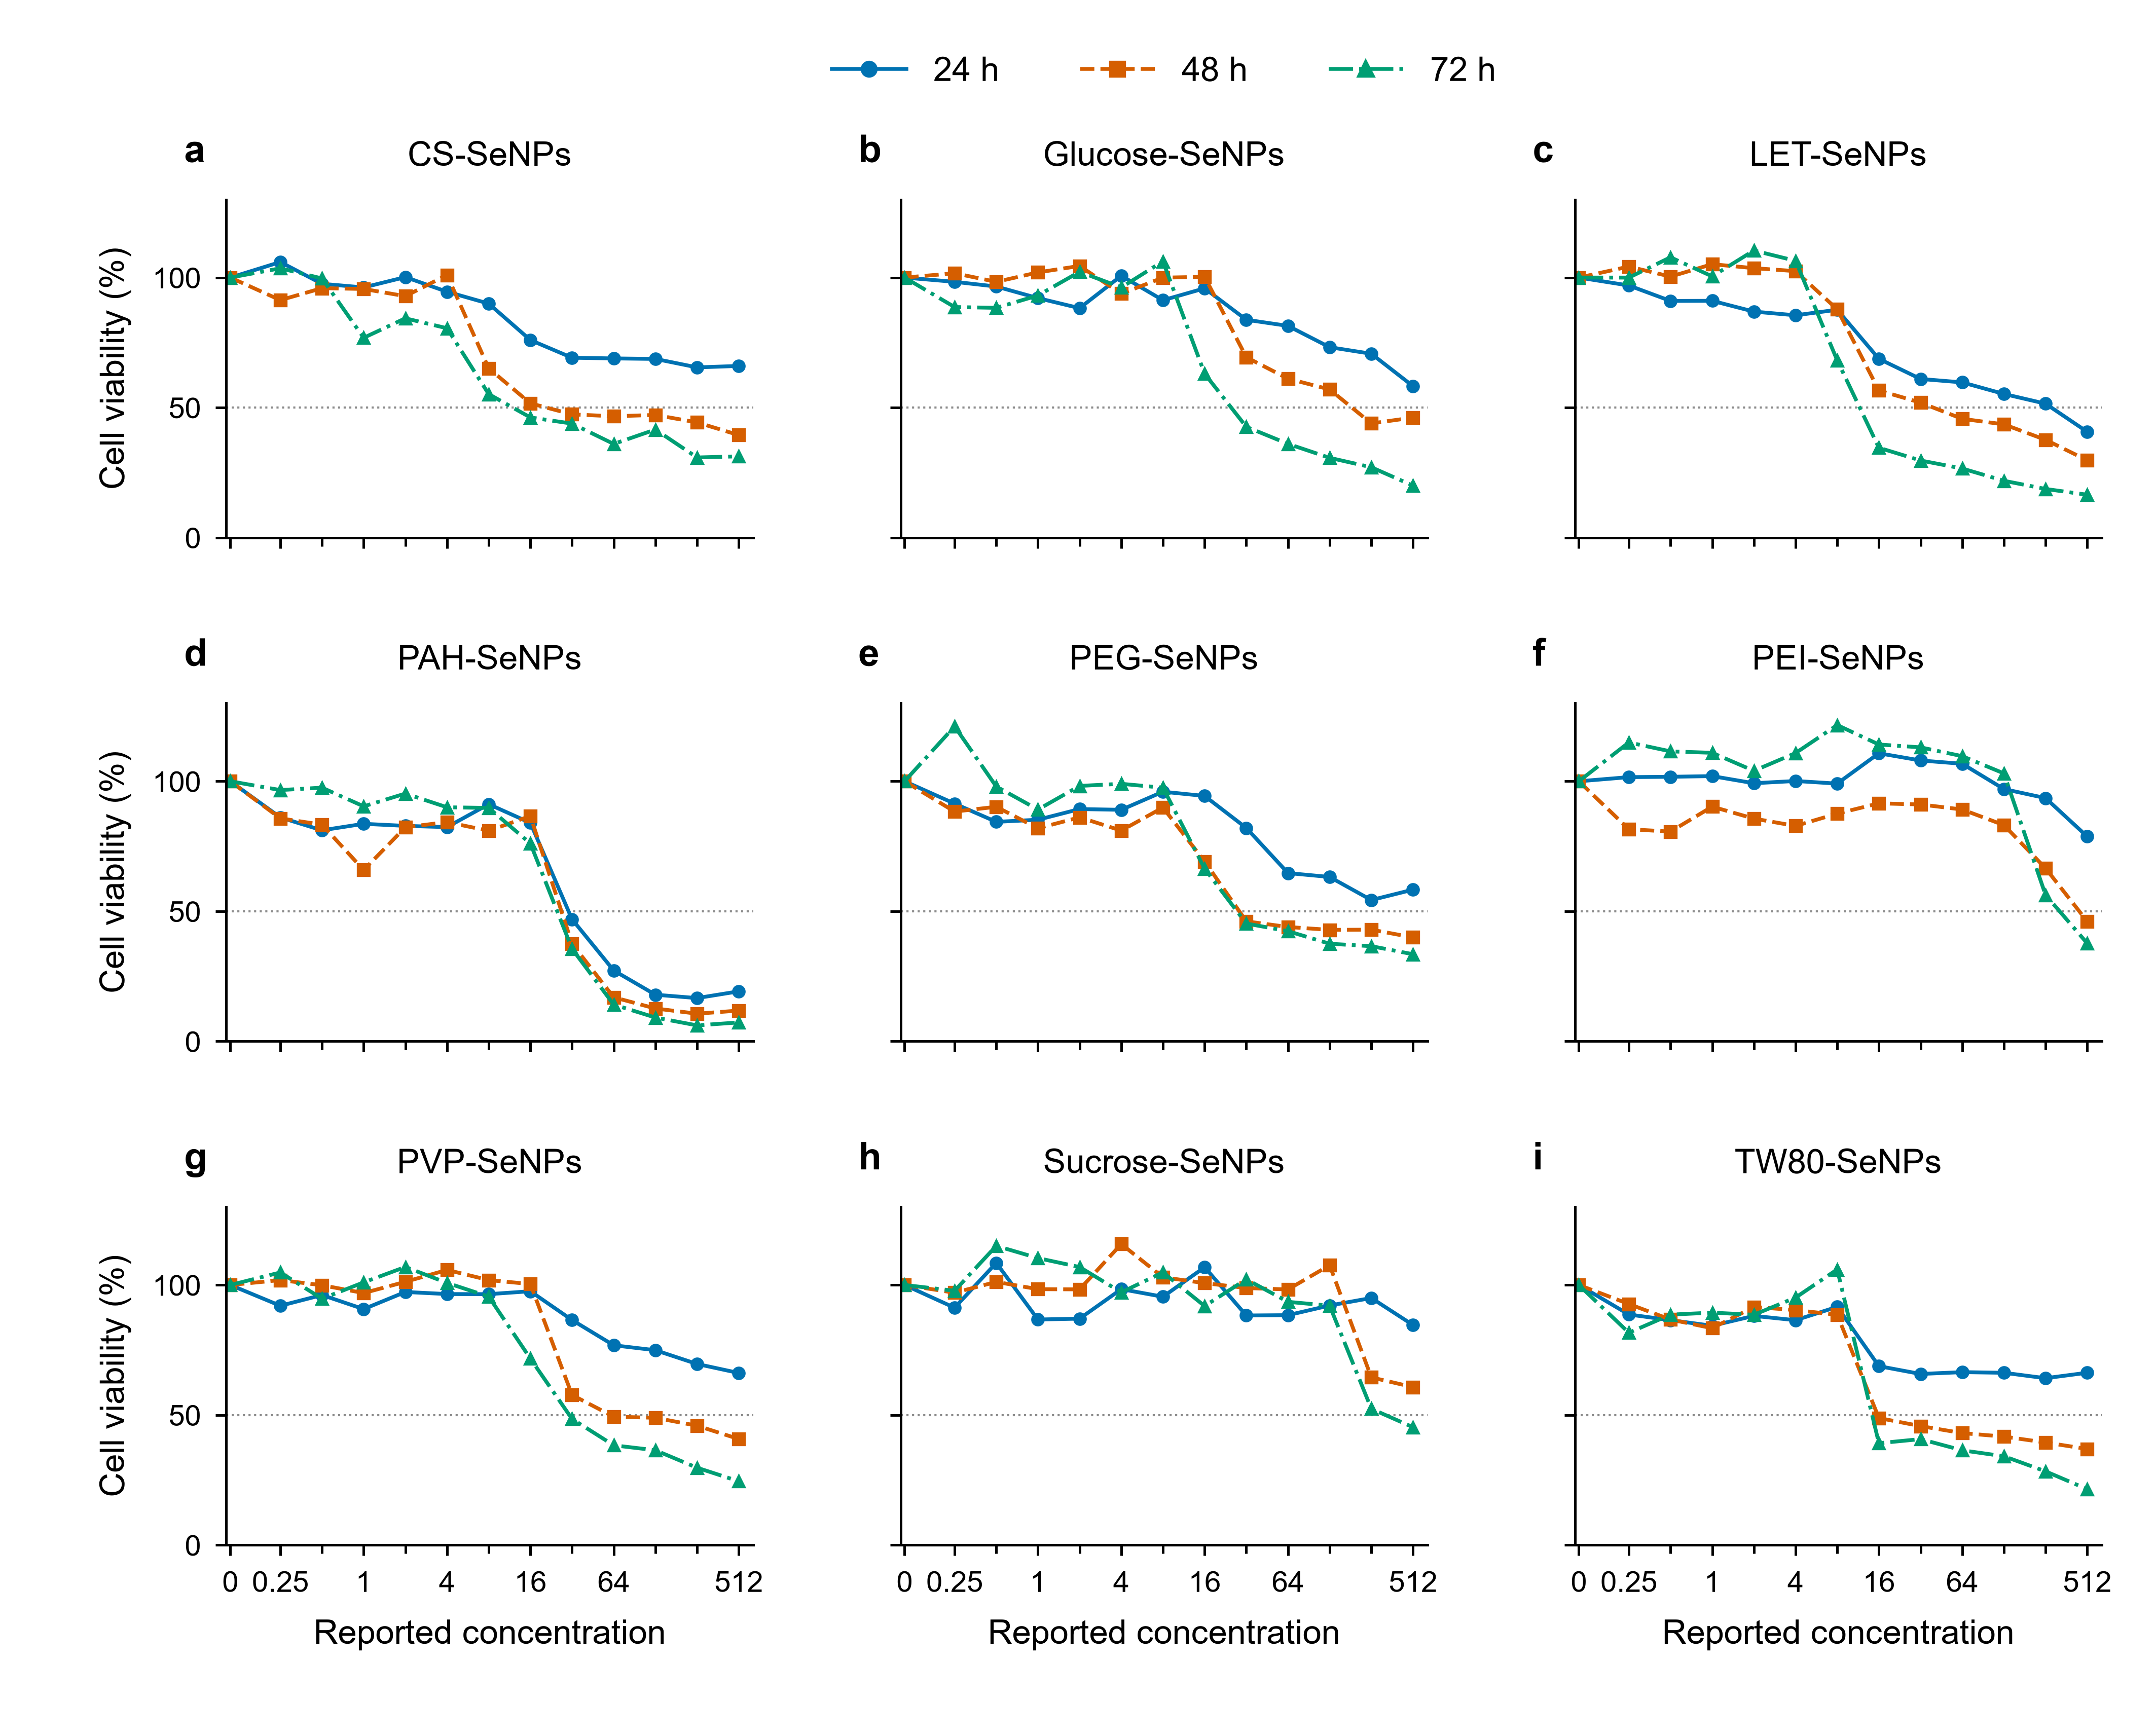
\includegraphics[width=\linewidth,height=0.70\textheight,keepaspectratio]{figures/huvec-dose-time.png}
\caption{9 种 SeNPs 在 HUVEC 中的剂量—时间报告曲线。a—i 依次为 CS、Glucose、LET、PAH、PEG、PEI、PVP、Sucrose 与 TW80。每个点为一个条件报告值，连线只连接报告点，虚线表示 50\% 存活率。浓度单位和计量基准待核实。}
\label{fig:huvec_dose_time}
\end{figure}

在报告浓度 512 下，以 9 种材料为分析单位，粒径与 24、48、72 h 存活率的 Spearman 系数分别为 0.200、0.383 和 0.267，Zeta 电位对应值为 0.050、\ensuremath{\mathord{-}}0.183 和 \ensuremath{\mathord{-}}0.050。这些描述性系数没有形成稳定的单变量关联证据，当前记录也不能区分粒径、电位、修饰化学及其他未测量因素的独立作用。依据冻结预测文件，已完成 351 个条件的预测—实测配对评价，并对 72 h、报告浓度 512 下的材料排序进行比较。

\subsection{冻结模型对新材料的存活率预测误差}

在351个材料—浓度—时间条件上，冻结模型预测与实验观测的总体 MAE 为 14.51 个存活率百分点，RMSE 为 20.11 个百分点，R\textsuperscript{2} 为 0.447，平均偏差为 +7.24 个百分点，表明模型在当前条件表中整体倾向于高估存活率（表~\ref{tab:huvec_external_performance}，图~\ref{fig:huvec_external_scatter}）。分时间点分析显示，24 h 的 MAE 和 RMSE 分别为 9.98 和 14.27 个百分点，48 h 分别为 13.99 和 18.86 个百分点，72 h 分别为 19.55 和 25.57 个百分点。预测误差随暴露时间延长而增大，提示模型未能充分捕捉较长暴露时间下的存活率下降。

在报告浓度 512 下，实验平均存活率在 24、48、72 h 分别为 59.81\%、39.07\% 和 26.38\%，模型预测均值则为 56.16\%、55.42\% 和 55.28\%。模型预测均值随时间变化较小，与实验观测的下降幅度不一致。上述结论限定于当前 9 种材料、HUVEC 体系和当前浓度映射，不能直接推广到其他细胞类型或材料。

\begin{table}[H]
\centering
\caption{冻结模型在 351 个 HUVEC 条件上的预测—实测误差。各条件不是独立实验重复。}
\label{tab:huvec_external_performance}
\small
\begin{tabular}{lrrrrr}
\toprule
时间 & n & MAE & RMSE & 预测均值 & 实测均值 \\
\midrule
24 h & 117 & 9.98 & 14.27 & 85.53 & 83.44 \\
48 h & 117 & 13.99 & 18.86 & 84.79 & 75.95 \\
72 h & 117 & 19.55 & 25.57 & 84.77 & 73.99 \\
总体 & 351 & 14.51 & 20.11 & 85.03 & 77.79 \\
\bottomrule
\end{tabular}

\end{table}

注：MAE、RMSE 的单位均为存活率百分点，均值单位为百分比。

\begin{figure}[H]
\centering
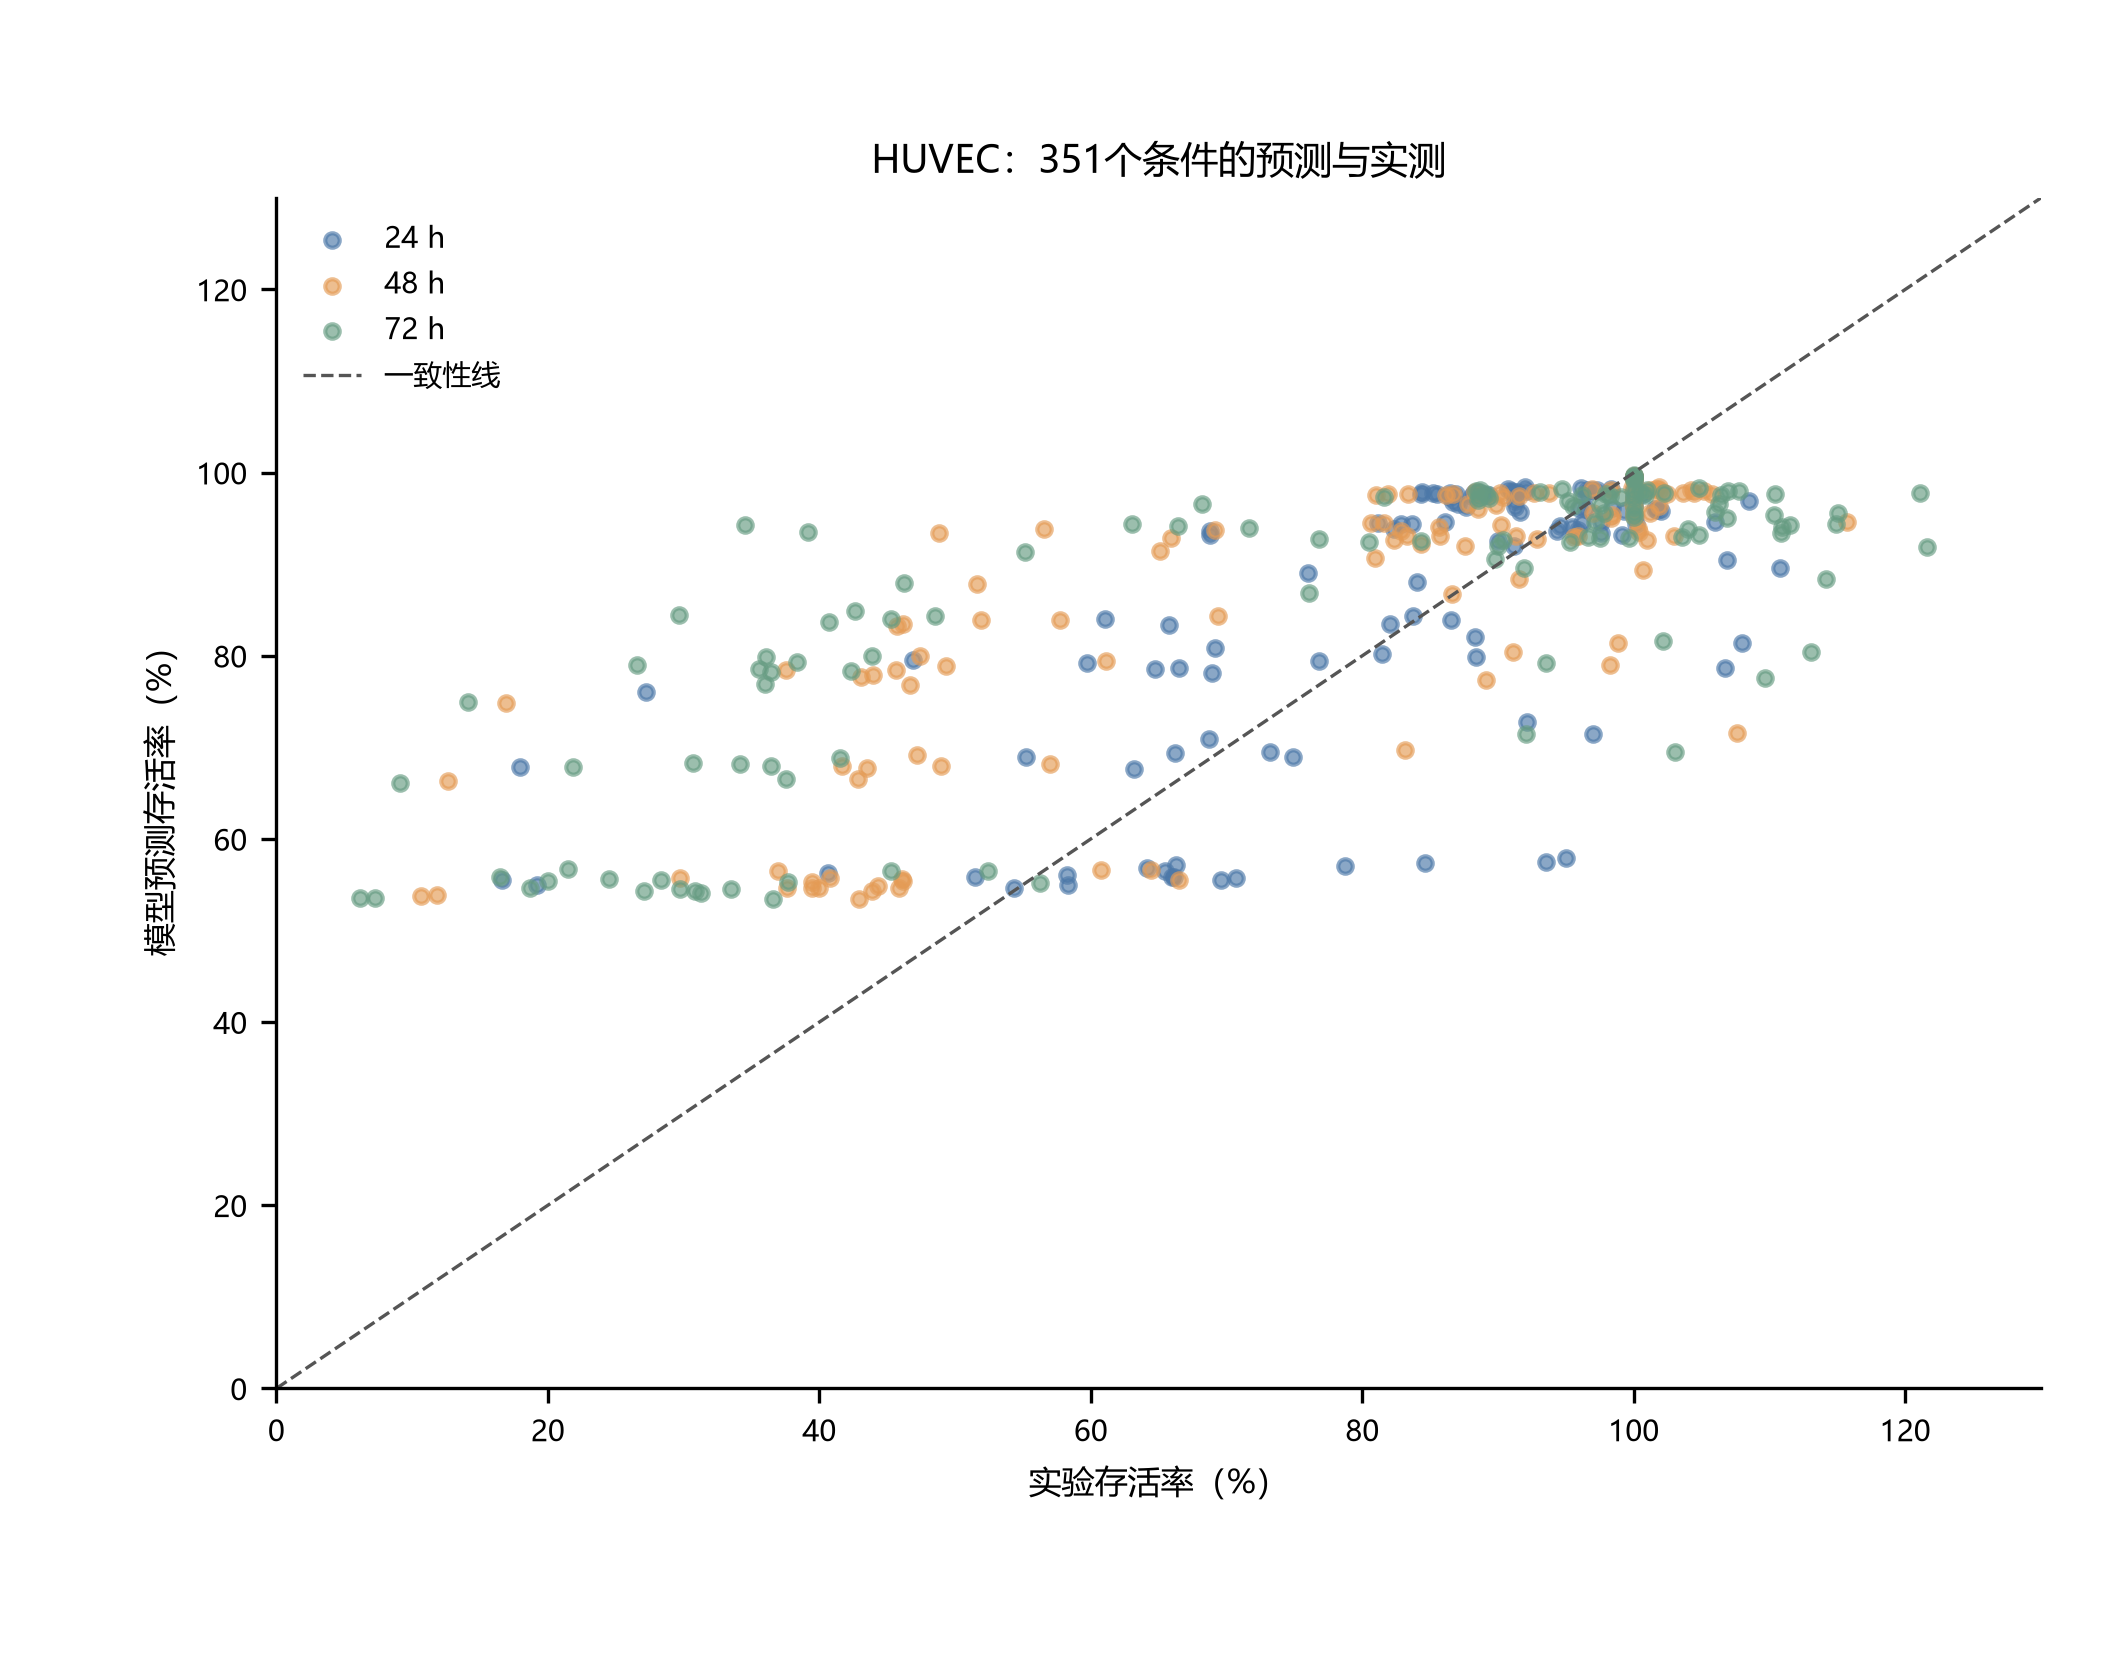
\includegraphics[width=\linewidth,height=0.70\textheight,keepaspectratio]{figures/scatter-viability.png}
\caption{冻结模型预测存活率与实验观测存活率的配对比较。虚线表示理想一致性线，颜色区分 24、48 和 72 h。}
\label{fig:huvec_external_scatter}
\end{figure}

\subsection{预测与实验毒性排序的一致性}

如图~\ref{fig:huvec_external_rank} 所示，在 HUVEC、72 h、报告浓度 512 的条件下，实验存活率从 PAH-SeNPs 的 7.26\% 到 Sucrose-SeNPs 的 45.30\%，跨度为 38.04 个百分点。相同条件下模型预测存活率集中在 53.54\% 至 56.69\% 之间，未能再现实验观测到的材料间差异。预测与实测排序的 Spearman 相关系数为 0.133，p = 0.732；Kendall \ensuremath{\tau} 为 0.111，p = 0.761。两项统计量均未显示可靠的排序一致性证据。由于分析单位为 9 种材料，结果应视为该指定条件下的描述性比较。

\begin{figure}[H]
\centering
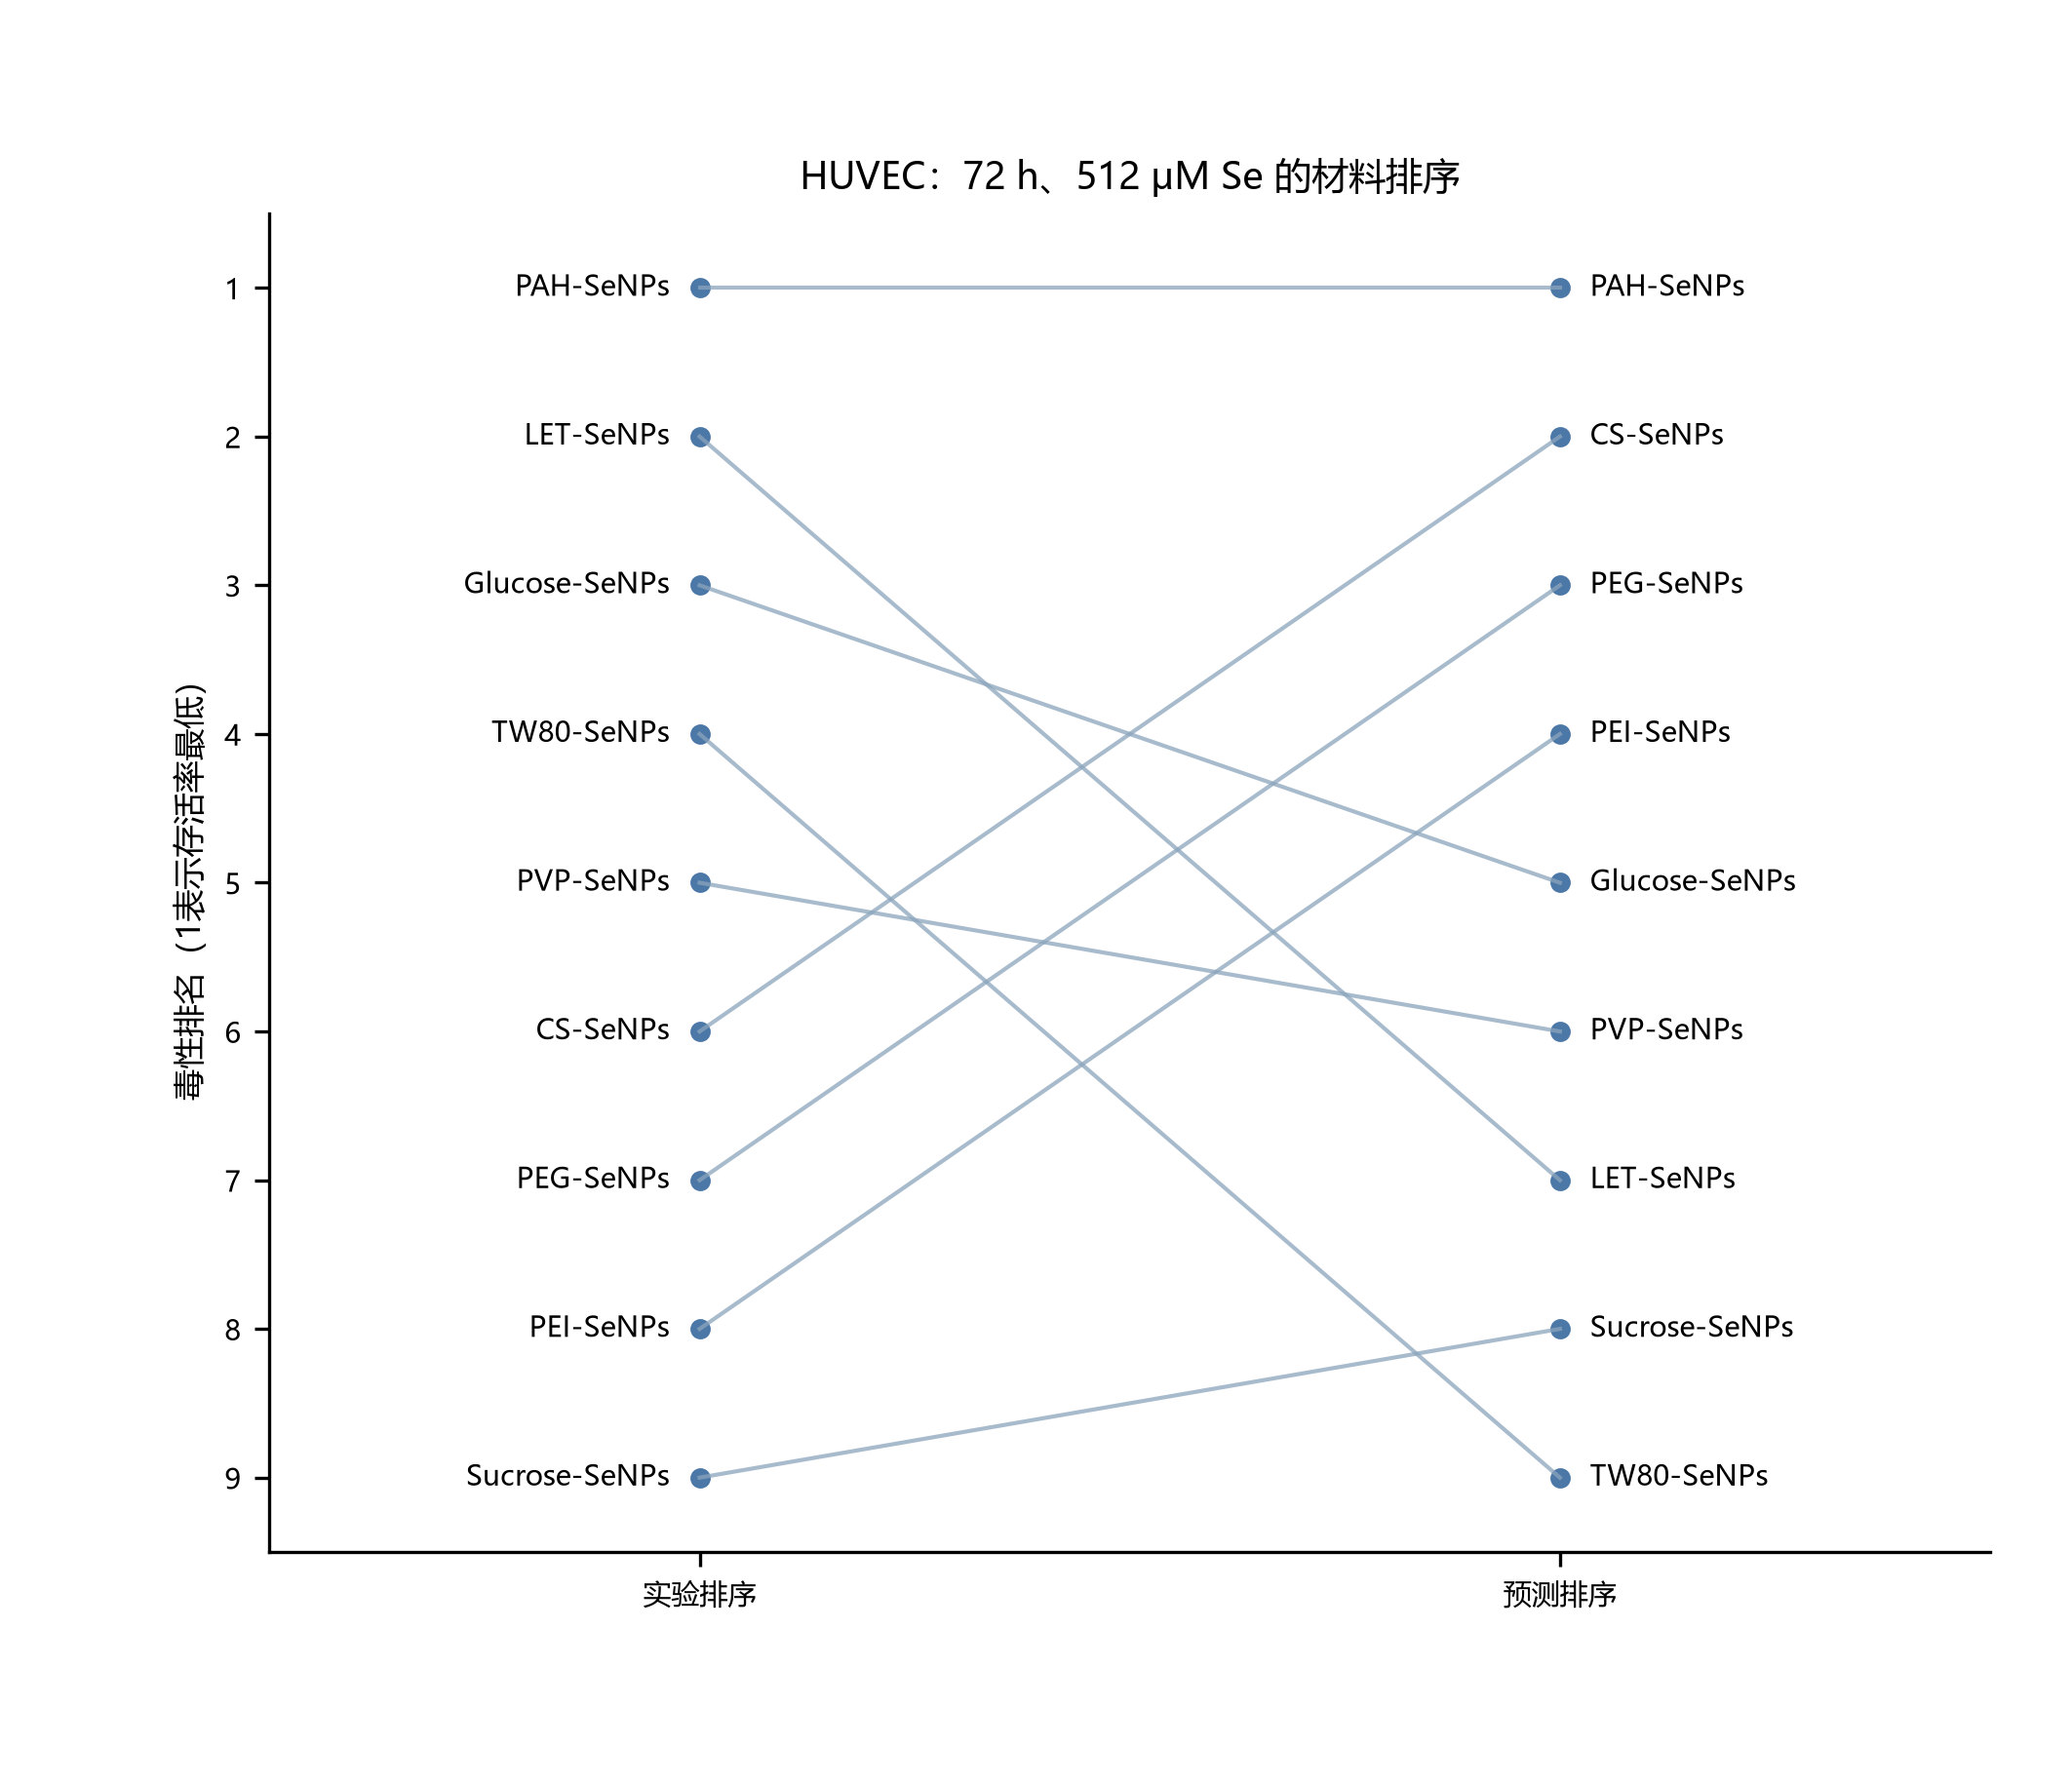
\includegraphics[width=\linewidth,height=0.70\textheight,keepaspectratio]{figures/rank-consistency.png}
\caption{72 h、报告浓度 512 下九种 SeNPs 的实验与预测毒性排序。排名 1 表示存活率最低、表观毒性最高，排名 9 表示存活率最高。}
\label{fig:huvec_external_rank}
\end{figure}

\subsection{粒径与 Zeta 电位的 SHAP 贡献}

图~\ref{fig:huvec_external_shap} 的 SHAP Summary Plot 展示了冻结随机森林对粒径组和 Zeta 相关特征组的预测贡献。图中各点代表一个材料—浓度—时间预测条件，横坐标为对预测存活率的有符号贡献，颜色表示相应描述符取值的高低。Zeta 组的贡献分布范围较宽，粒径组也呈现随条件变化的正负贡献。该结果说明模型在不同预测条件下使用这些特征的方式并不相同，但 SHAP 贡献反映的是模型内部的预测分配，不能解释为粒径或 Zeta 电位对细胞毒性的因果效应。

\begin{figure}[H]
\centering
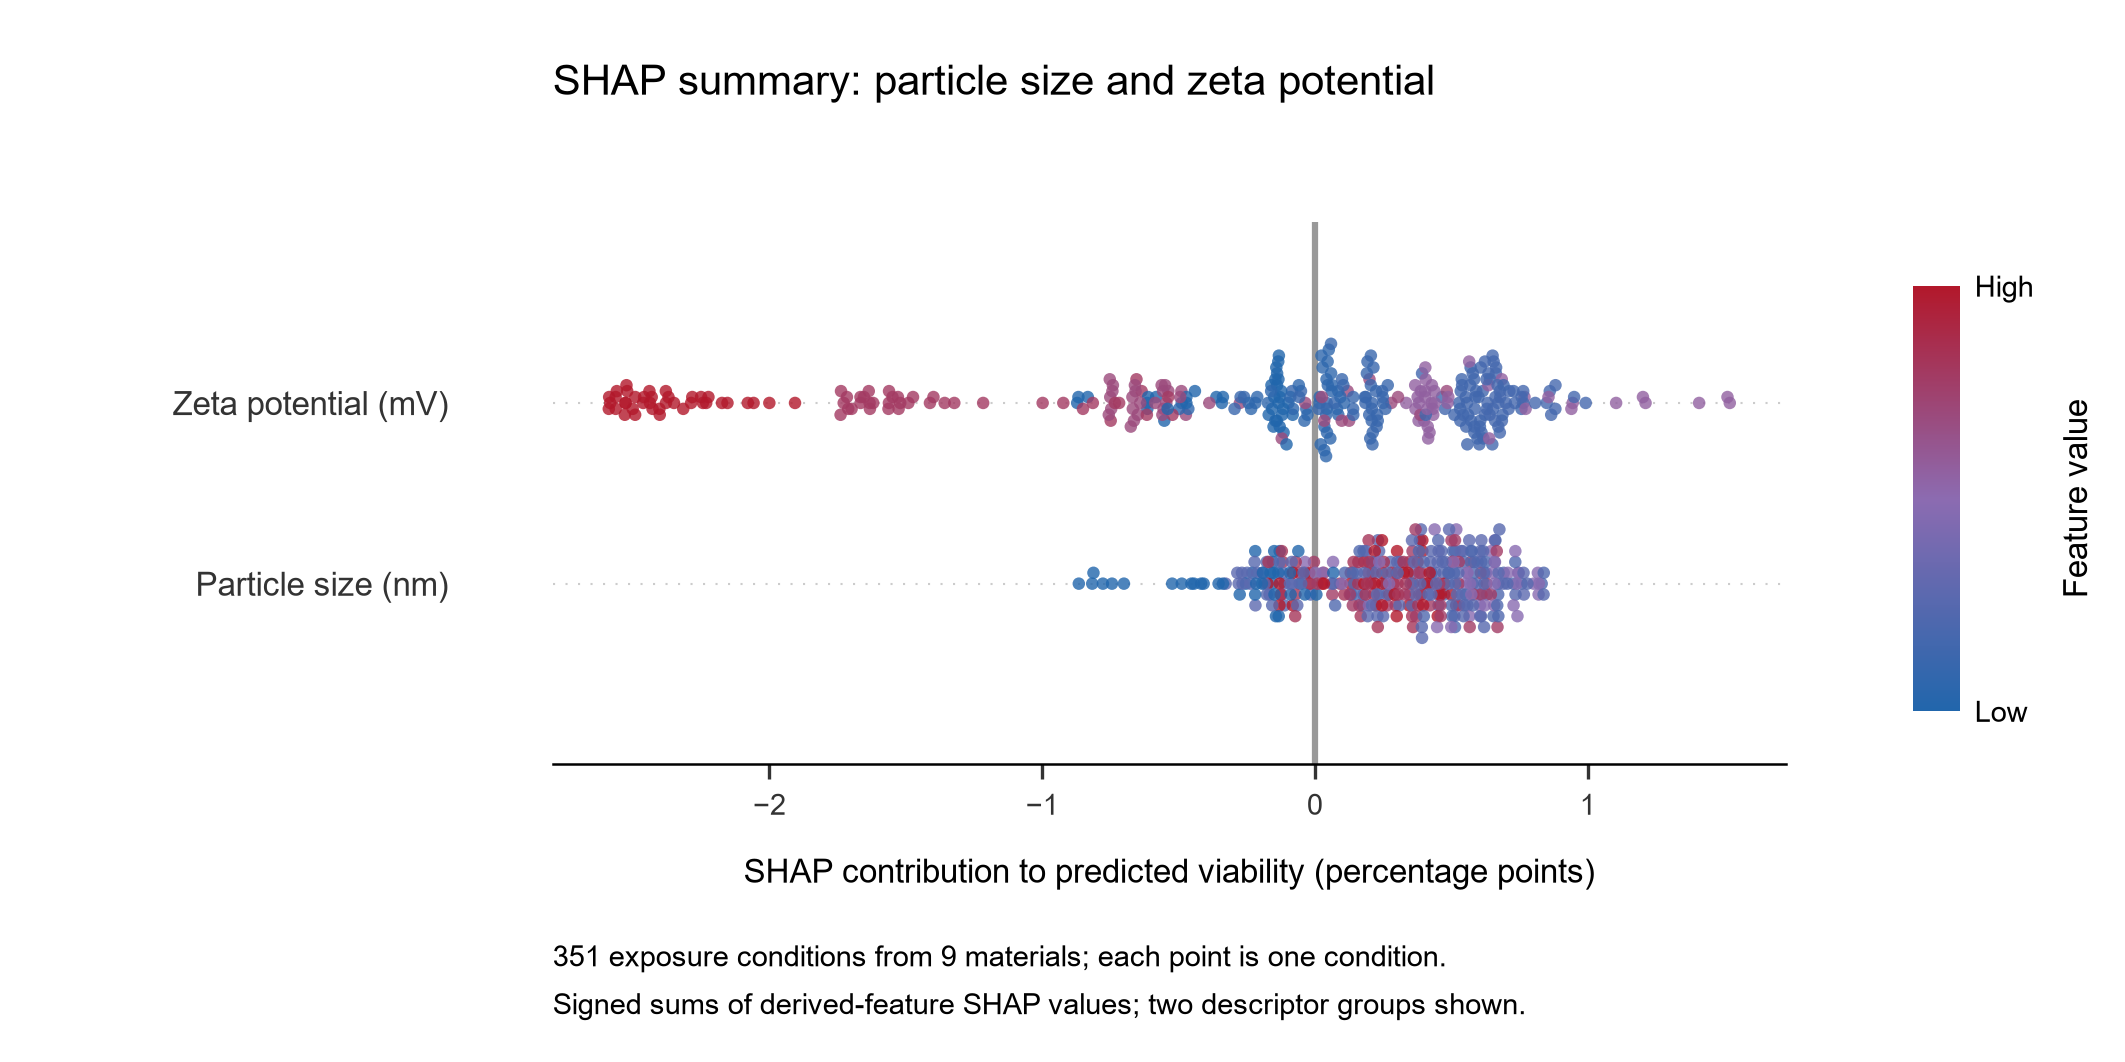
\includegraphics[width=\linewidth,height=0.70\textheight,keepaspectratio]{figures/shap-summary.png}
\caption{冻结随机森林模型中粒径与 Zeta 电位相关特征组的 SHAP Summary Plot。每个点为一个预测条件，不代表独立实验重复。}
\label{fig:huvec_external_shap}
\end{figure}

\subsection{预测问题的界定与材料信息的实际增量}

本研究把历史模型评价和新增实验观测置于同一研究问题下，同时保留两者不同的证据任务。历史分组结果显示，当前基础输入对跨文献存活率的预测仍有较大误差，更多化学字段、显式剂量—时间交互与固定预算迁移没有稳定降低误差；新增实验则提供了真实材料在 HUVEC 中的响应曲线，展示了时间变化与条件相关的材料差异。两部分共同说明，预测性能和实验响应结构需要各自获得直接证据，方向一致的实验趋势不足以替代逐样本预测评价。

化学增强的阴性结果限定于当前字段质量、样本组成与模型配置，并不说明材料化学性质在毒性形成中没有作用。历史数据的 Zeta 电位缺失率为 42.40\%，修饰物类别和分子量没有完整字段，晶体信息编码又只反映是否报告晶体学信息，这些条件限制了模型对材料差异的识别。表征方法、报告习惯和研究环境还可能共同影响输入值，新增字段是否具有生物学意义，与其能否在当前归档数据中提供稳定预测增量，属于需要分开讨论的问题。

同样，迁移对照尚未建立稳定收益，可能与不同材料体系的响应分布、共同特征的覆盖以及当前树模型迁移接口有关。RF 的新增树训练保留原有通用树，XGBoost 的续训依赖已学习的通用结构，本研究没有检验其他迁移方法，不能将结果推广为迁移学习对 SeNPs 普遍无效。对于现阶段的材料筛选，更合适的工作是明确模型可接受的输入、记录外部测试条件，并检验预测误差，而不是根据通用基准指标直接判断新材料预测精度。

\subsection{与既有计算研究的关系}

Gul 等的跨材料属性分析与 Masarkar 等的预测研究，为组织纳米材料理化性质、细胞背景和暴露条件提供了基础 \cite{gul2021association,masarkar2024}。本研究进一步关注这些信息在 SeNPs 文献分组评价下的增量，以及新增实验如何与历史建模衔接。由于数据纳入、特征定义、模型选择与验证划分均不同，本研究不以跨论文的单个 $R^2$ 或 MAE 数值宣称性能优于既有工作，早期深度模型指标作为历史探索保留，不纳入后续分组评价的统一模型排名。

嵌套评价使内层选择与外层报告分离，对有限样本下模型选择偏差的控制与已有方法学研究一致 \cite{cawley2010selection}。不过，文献分组验证只检验对未参与训练的文献组的表现，不能自动代表对未知配方、未知修饰物或不同实验室的泛化。旧历史复现还混合了随机交叉验证误差、全量拟合 $R^2$ 和不同预处理设置，当前结果不构成只改变划分方式的受控对照，因此性能差异不能全部归因于随机划分造成的泄漏，方法与数据口径的变化也需要保留在解释中。

\subsection{实验观测的意义与机制解释范围}

HUVEC 数据把研究从历史文献预测扩展到真实材料的剂量—时间观测，最高测试浓度下的时间变化与有限 IC50 估计数量的增加共同表明，评价时间会影响材料差异的呈现方式。对照已有SeNPs 细胞研究，这些结果支持将材料修饰和暴露条件一起纳入实验比较 \cite{wang2020prooxidation,lunkov2023chitosan}，但当前单一细胞模型不能提供正常与肿瘤细胞选择性、跨细胞普适性或体内安全性的证据。

材料的高浓度排序与表观 IC50 排序并不一致，反映了固定浓度残余存活率与跨越 50\% 阈值所处位置的不同。表观 IC50 仅由两个相邻报告点插值，浓度间距、局部波动和检测读数都可能影响估计，尚不能用于给出精细的材料优劣判断。对没有跨越阈值的曲线保留 > 512 状态，也避免了在测试范围外强行拟合一个看似完整的数值。

粒径、电位和修饰信息在不同材料之间同时变化，每种材料又仅有一组描述符报告值，因此弱秩相关既不能证明这些性质无作用，也不能将某种材料的低存活率归因于单个描述符。大于 100\%的报告值同样需要谨慎解释，当前缺少原始孔读数、空白扣除及检测干扰信息，不能据此判定真实增殖促进或特定毒性机制。核对这些实验信息后，才能进一步评估剂量曲线的波动与材料相关的检测影响。

\subsection{外部预测评价仍需完成的环节}

按材料、报告浓度、时间及浓度单位匹配后获得 351 对预测—实测值，因而本研究可以报告当前条件表上的 MAE、RMSE、平均偏差及预测—实测排序一致性。每个条件只有一个归档报告值，不能据此估计独立实验重复间的变异。实测 IC50 不能作为新材料初筛模型的输入。

\section{结论}

%本文在通用纳米颗粒基准比较、纳米硒专用建模、增强特征筛选和多模态融合的早期研究基础上，加入了文献分组验证与独立 HUVEC 实验评价。来自 43 篇文献的 383 条早期记录支持了模型与特征组合的探索；另一份归档工作簿中的 434 条记录%用于严格分组评价，两者的数据纳入、预处理和指标口径不同，不能直接合并或将其性能差异全部归因于某一验证策略。

%早期含 IC50 的增强 XGBoost 取得三折交叉验证 MAE 7.20 个百分点和全量拟合 $R^2=0.957$，该结果保留为响应相关辅助分析。后续不含实测 IC50 的随机森林基础模型在文献分组嵌套评价中的折外 MAE 为 19.11 个百分点，当前化学增强、剂量—时间交互及固定预算迁移未显示稳定改善。因此，材料化学描述符具有继续采集与检验的价值，但现有证据不足以证明其已带来可迁移的独立收益，也不足以根据历史拟合指标确定部署模型。

%新增九种 SeNPs 的 351 个 HUVEC 条件报告值，将原有外部验证计划推进到逐条件预测—实测比较。冻结模型的总体 MAE 为 14.51 个百分点、RMSE 为 20.11 个百分点、$R^2=0.447$，但对较长暴露时间的误差增大，预测材料排序与实测一致性较低。实验的 27 条曲线中 19 条可估计表观 IC50、8 条未达到阈值，而预测曲线均未跨越 50\% 存活率。SHAP 分析说明模型如何使用粒径和 Zeta 相关特征，不能替代材料性质的因果验证。

%研究由此形成了从文献整理、模型比较和特征工程到严格分组评价及实验检验的连续路径。下一步需要核对浓度计量与换算基准、补齐实验流程和重复数据，并在独立材料或批次中检验模型冻结、预测与解盲过程。在这些条件得到验证前，当前模型适合作为进一步研究的基线，尚不能据此直接判定新材料安全性、可靠毒性排序或有限 IC50。




本文围绕纳米硒细胞毒性预测，结合文献数据建模、按文献来源分组的交叉验证和 HUVEC 实验，考察材料性质与暴露条件对细胞存活率预测的作用。在筛选后的 434 条数据上，不使用实测 IC50 作为输入的随机森林基础模型，其交叉验证 MAE 为 19.11。加入材料化学特征、浓度与暴露时间交互项及采用迁移学习方案，在当前数据和模型设置下未获得稳定的性能提升。结果表明，模型对不同文献来源数据的预测精度仍有待提高，材料化学特征的预测价值需要结合更完整的数据进一步评价。

将保存的预测结果与 9 种纳米硒材料在 351 个 HUVEC 实验条件下的实测值进行比较，得到 MAE 为 14.51、RMSE 为 20.11、$R^2$ 为 0.447。预测结果虽然整体偏高，但是能够反映部分存活率差异。实验结果为比较不同材料在各暴露条件下的细胞毒性提供了依据，并指出了存活率预测和 IC50 估计中需要改进的问题。

本研究为依据材料性质和暴露条件预测纳米硒细胞毒性提供了研究基础，模型用于实验前材料筛选的可靠性仍需进一步验证。后续将完善材料表征与实验重复数据，统一浓度计量和换算依据，并在更多材料、独立批次及不同细胞体系中检验预测效果，以提高模型对暴露时间变化和材料间毒性差异的预测能力。


\section*{Acknowledgements}

Please use ``The authors thank \ldots'' rather than ``The authors would like to
thank \ldots''.

\clearpage
\section*{补充材料}
\begingroup
\setcounter{table}{0}
\renewcommand{\thetable}{S\arabic{table}}
\small
\setlength{\tabcolsep}{3.5pt}
\setlength{\LTleft}{0pt}
\setlength{\LTright}{0pt}
\renewcommand{\arraystretch}{1.12}
\begin{longtable}{r >{\raggedright\arraybackslash}p{0.21\linewidth} >{\raggedright\arraybackslash}p{0.66\linewidth}}
\caption{纳米硒专用数据集的来源文献（43 篇，2008--2022 年）。}\label{tab:source-publications}\\
\toprule
序号 & 来源文献 & 文献题名与 DOI \\
\midrule
\endfirsthead
\multicolumn{3}{l}{表 S1（续）} \\
\toprule
序号 & 来源文献 & 文献题名与 DOI \\
\midrule
\endhead
\midrule
\multicolumn{3}{r}{续下页} \\
\endfoot
\bottomrule
\endlastfoot
% 中英文共用同一组文献键；题名、作者、年份和 DOI 均由 references.bib 提供。
1 & \citeauthor{chen_selenium_2008} (\citeyear{chen_selenium_2008})~\cite{chen_selenium_2008} & \citetitle{chen_selenium_2008}\newline\citefield{chen_selenium_2008}{doi} \\
\addlinespace[4pt]
2 & \citeauthor{li_reversal_2011} (\citeyear{li_reversal_2011})~\cite{li_reversal_2011} & \citetitle{li_reversal_2011}\newline\citefield{li_reversal_2011}{doi} \\
\addlinespace[4pt]
3 & \citeauthor{zheng_sialic_2011} (\citeyear{zheng_sialic_2011})~\cite{zheng_sialic_2011} & \citetitle{zheng_sialic_2011}\newline\citefield{zheng_sialic_2011}{doi} \\
\addlinespace[4pt]
4 & \citeauthor{liu_selenium_2012} (\citeyear{liu_selenium_2012})~\cite{liu_selenium_2012} & \citetitle{liu_selenium_2012}\newline\citefield{liu_selenium_2012}{doi} \\
\addlinespace[4pt]
5 & \citeauthor{wu_surface_2012} (\citeyear{wu_surface_2012})~\cite{wu_surface_2012} & \citetitle{wu_surface_2012}\newline\citefield{wu_surface_2012}{doi} \\
\addlinespace[4pt]
6 & \citeauthor{chen_surface_2012} (\citeyear{chen_surface_2012})~\cite{chen_surface_2012} & \citetitle{chen_surface_2012}\newline\citefield{chen_surface_2012}{doi} \\
\addlinespace[4pt]
7 & \citeauthor{yu_positive_2012} (\citeyear{yu_positive_2012})~\cite{yu_positive_2012} & \citetitle{yu_positive_2012}\newline\citefield{yu_positive_2012}{doi} \\
\addlinespace[4pt]
8 & \citeauthor{chen_peg-nanolized_2012} (\citeyear{chen_peg-nanolized_2012})~\cite{chen_peg-nanolized_2012} & \citetitle{chen_peg-nanolized_2012}\newline\citefield{chen_peg-nanolized_2012}{doi} \\
\addlinespace[4pt]
9 & \citeauthor{pi_pathway_2013} (\citeyear{pi_pathway_2013})~\cite{pi_pathway_2013} & \citetitle{pi_pathway_2013}\newline\citefield{pi_pathway_2013}{doi} \\
\addlinespace[4pt]
10 & \citeauthor{wu_induction_2013} (\citeyear{wu_induction_2013})~\cite{wu_induction_2013} & \citetitle{wu_induction_2013}\newline\citefield{wu_induction_2013}{doi} \\
\addlinespace[4pt]
11 & \citeauthor{feng_differential_2014} (\citeyear{feng_differential_2014})~\cite{feng_differential_2014} & \citetitle{feng_differential_2014}\newline\citefield{feng_differential_2014}{doi} \\
\addlinespace[4pt]
12 & \citeauthor{huang_selective_2013} (\citeyear{huang_selective_2013})~\cite{huang_selective_2013} & \citetitle{huang_selective_2013}\newline\citefield{huang_selective_2013}{doi} \\
\addlinespace[4pt]
13 & \citeauthor{li_functionalized_2013} (\citeyear{li_functionalized_2013})~\cite{li_functionalized_2013} & \citetitle{li_functionalized_2013}\newline\citefield{li_functionalized_2013}{doi} \\
\addlinespace[4pt]
14 & \citeauthor{zhang_enhancement_2013} (\citeyear{zhang_enhancement_2013})~\cite{zhang_enhancement_2013} & \citetitle{zhang_enhancement_2013}\newline\citefield{zhang_enhancement_2013}{doi} \\
\addlinespace[4pt]
15 & \citeauthor{jiang_gracilaria_2014} (\citeyear{jiang_gracilaria_2014})~\cite{jiang_gracilaria_2014} & \citetitle{jiang_gracilaria_2014}\newline\citefield{jiang_gracilaria_2014}{doi} \\
\addlinespace[4pt]
16 & \citeauthor{yu_ph-responsive_2014} (\citeyear{yu_ph-responsive_2014})~\cite{yu_ph-responsive_2014} & \citetitle{yu_ph-responsive_2014}\newline\citefield{yu_ph-responsive_2014}{doi} \\
\addlinespace[4pt]
17 & \citeauthor{zeng_construction_2015} (\citeyear{zeng_construction_2015})~\cite{zeng_construction_2015} & \citetitle{zeng_construction_2015}\newline\citefield{zeng_construction_2015}{doi} \\
\addlinespace[4pt]
18 & \citeauthor{liu_sequentially_2016} (\citeyear{liu_sequentially_2016})~\cite{liu_sequentially_2016} & \citetitle{liu_sequentially_2016}\newline\citefield{liu_sequentially_2016}{doi} \\
\addlinespace[4pt]
19 & \citeauthor{liu_facile_2016} (\citeyear{liu_facile_2016})~\cite{liu_facile_2016} & \citetitle{liu_facile_2016}\newline\citefield{liu_facile_2016}{doi} \\
\addlinespace[4pt]
20 & \citeauthor{yu_x-ray-responsive_2016} (\citeyear{yu_x-ray-responsive_2016})~\cite{yu_x-ray-responsive_2016} & \citetitle{yu_x-ray-responsive_2016}\newline\citefield{yu_x-ray-responsive_2016}{doi} \\
\addlinespace[4pt]
21 & \citeauthor{fu_rgd_2016} (\citeyear{fu_rgd_2016})~\cite{fu_rgd_2016} & \citetitle{fu_rgd_2016}\newline\citefield{fu_rgd_2016}{doi} \\
\addlinespace[4pt]
22 & \citeauthor{fang_targeting_2017} (\citeyear{fang_targeting_2017})~\cite{fang_targeting_2017} & \citetitle{fang_targeting_2017}\newline\citefield{fang_targeting_2017}{doi} \\
\addlinespace[4pt]
23 & \citeauthor{chen_efficient_2018} (\citeyear{chen_efficient_2018})~\cite{chen_efficient_2018} & \citetitle{chen_efficient_2018}\newline\citefield{chen_efficient_2018}{doi} \\
\addlinespace[4pt]
24 & \citeauthor{fang_dualtargeted_2018} (\citeyear{fang_dualtargeted_2018})~\cite{fang_dualtargeted_2018} & \citetitle{fang_dualtargeted_2018}\newline\citefield{fang_dualtargeted_2018}{doi} \\
\addlinespace[4pt]
25 & \citeauthor{huang_autophagy_2018} (\citeyear{huang_autophagy_2018})~\cite{huang_autophagy_2018} & \citetitle{huang_autophagy_2018}\newline\citefield{huang_autophagy_2018}{doi} \\
\addlinespace[4pt]
26 & \citeauthor{liu_highly_2018} (\citeyear{liu_highly_2018})~\cite{liu_highly_2018} & \citetitle{liu_highly_2018}\newline\citefield{liu_highly_2018}{doi} \\
\addlinespace[4pt]
27 & \citeauthor{wang_regulating_2016} (\citeyear{wang_regulating_2016})~\cite{wang_regulating_2016} & \citetitle{wang_regulating_2016}\newline\citefield{wang_regulating_2016}{doi} \\
\addlinespace[4pt]
28 & \citeauthor{hu_selenium_2019} (\citeyear{hu_selenium_2019})~\cite{hu_selenium_2019} & \citetitle{hu_selenium_2019}\newline\citefield{hu_selenium_2019}{doi} \\
\addlinespace[4pt]
29 & \citeauthor{zeng_potentiation_2019} (\citeyear{zeng_potentiation_2019})~\cite{zeng_potentiation_2019} & \citetitle{zeng_potentiation_2019}\newline\citefield{zeng_potentiation_2019}{doi} \\
\addlinespace[4pt]
30 & \citeauthor{huang_dual-targeting_2019} (\citeyear{huang_dual-targeting_2019})~\cite{huang_dual-targeting_2019} & \citetitle{huang_dual-targeting_2019}\newline\citefield{huang_dual-targeting_2019}{doi} \\
\addlinespace[4pt]
31 & \citeauthor{huang_highly_2019} (\citeyear{huang_highly_2019})~\cite{huang_highly_2019} & \citetitle{huang_highly_2019}\newline\citefield{huang_highly_2019}{doi} \\
\addlinespace[4pt]
32 & \citeauthor{zhang_systematic_2019} (\citeyear{zhang_systematic_2019})~\cite{zhang_systematic_2019} & \citetitle{zhang_systematic_2019}\newline\citefield{zhang_systematic_2019}{doi} \\
\addlinespace[4pt]
33 & \citeauthor{zheng_thermosensitive_2019} (\citeyear{zheng_thermosensitive_2019})~\cite{zheng_thermosensitive_2019} & \citetitle{zheng_thermosensitive_2019}\newline\citefield{zheng_thermosensitive_2019}{doi} \\
\addlinespace[4pt]
34 & \citeauthor{huang_chiralitydriven_2020} (\citeyear{huang_chiralitydriven_2020})~\cite{huang_chiralitydriven_2020} & \citetitle{huang_chiralitydriven_2020}\newline\citefield{huang_chiralitydriven_2020}{doi} \\
\addlinespace[4pt]
35 & \citeauthor{yang_lentinan-functionalized_2020} (\citeyear{yang_lentinan-functionalized_2020})~\cite{yang_lentinan-functionalized_2020} & \citetitle{yang_lentinan-functionalized_2020}\newline\citefield{yang_lentinan-functionalized_2020}{doi} \\
\addlinespace[4pt]
36 & \citeauthor{liu_rapid_2021} (\citeyear{liu_rapid_2021})~\cite{liu_rapid_2021} & \citetitle{liu_rapid_2021}\newline\citefield{liu_rapid_2021}{doi} \\
\addlinespace[4pt]
37 & \citeauthor{an_functionalized_2021} (\citeyear{an_functionalized_2021})~\cite{an_functionalized_2021} & \citetitle{an_functionalized_2021}\newline\citefield{an_functionalized_2021}{doi} \\
\addlinespace[4pt]
38 & \citeauthor{song_translational_2021} (\citeyear{song_translational_2021})~\cite{song_translational_2021} & \citetitle{song_translational_2021}\newline\citefield{song_translational_2021}{doi} \\
\addlinespace[4pt]
39 & \citeauthor{yang_atherosclerotic_2022} (\citeyear{yang_atherosclerotic_2022})~\cite{yang_atherosclerotic_2022} & \citetitle{yang_atherosclerotic_2022}\newline\citefield{yang_atherosclerotic_2022}{doi} \\
\addlinespace[4pt]
40 & \citeauthor{yang_functionalized_2021} (\citeyear{yang_functionalized_2021})~\cite{yang_functionalized_2021} & \citetitle{yang_functionalized_2021}\newline\citefield{yang_functionalized_2021}{doi} \\
\addlinespace[4pt]
41 & \citeauthor{liang_translational_2022} (\citeyear{liang_translational_2022})~\cite{liang_translational_2022} & \citetitle{liang_translational_2022}\newline\citefield{liang_translational_2022}{doi} \\
\addlinespace[4pt]
42 & \citeauthor{liu_specific_2022} (\citeyear{liu_specific_2022})~\cite{liu_specific_2022} & \citetitle{liu_specific_2022}\newline\citefield{liu_specific_2022}{doi} \\
\addlinespace[4pt]
43 & \citeauthor{du_highly_2022} (\citeyear{du_highly_2022})~\cite{du_highly_2022} & \citetitle{du_highly_2022}\newline\citefield{du_highly_2022}{doi} \\
\addlinespace[4pt]

\end{longtable}
\noindent \textit{注：}逐文献记录数尚待根据原始 383 条数据核实。书目信息由中英文共享的参考文献库提供。

\subsection{输入特征与参数候选}

基础配置的 19 个字段依次为：修饰/官能团信息、合成方法、表面电荷、细胞类型、细胞组织、发表年份、最终粒径、最终 Zeta 电位、Zeta 绝对值、暴露时间、历史浓度、log(1 + 粒径)、log(1 + 时间)、log(1 + 浓度)、接种细胞数，以及 Zeta、细胞数、修饰信息和表面电荷的四个缺失标志。化学候选为 Se 含量、稳定性时间、Se 3d 结合能和晶体学报告状态，IC50 配置额外考虑历史实测 IC50 。晶体学报告状态使用原晶体学字段是否非空构造，不是测定晶相的替代值。

RF 候选（树数、最大深度、叶节点最小样本数）为（250、不限、2）、（250、10、2）和（250、不限、4）；XGBoost 候选（轮次、最大深度、学习率）为（150、2、0.05）、（250、2、0.05）和（250、3、0.05）。固定预算通用与迁移对照使用 500 树预算，RF 的最小叶节点样本数为 2，XGBoost 的最大深度为 3、学习率为 0.05，其余固定参数与方法部分一致。

\subsection{完整配对增量结果}

表~\ref{tab:paired_comparisons} 同时列出样本等权差值与文献组等权差值，区间对应后者。基础嵌套分析中归档的逐样本 bootstrap 指标区间属于另一不确定性口径，本稿不将它们写成文献组区间，也不将通用基准中的组等权区间直接附到样本等权性能数值上。

\begin{table}[H]
\centering
\caption{各配置相对对应基线的配对 MAE 差值，单位为存活率百分点。负值表示误差下降，区间来自 24 个文献组等权差值的 5000 次 bootstrap。}
\label{tab:paired_comparisons}
\small
\begin{tabularx}{\linewidth}{lXrrr}
\toprule
模型 & 对照 & \ensuremath{\Delta}MAE 样本等权 & \ensuremath{\Delta}MAE 文献组等权 & 文献组等权 95\% 区间 \\
\midrule
RF & 化学增强 & +0.180 & +0.183 & [0.054, 0.333] \\
XGBoost & 化学增强 & +0.030 & \ensuremath{\mathord{-}}0.049 & [\ensuremath{\mathord{-}}0.822, 0.668] \\
RF & IC50 辅助 & \ensuremath{\mathord{-}}0.142 & \ensuremath{\mathord{-}}0.326 & [\ensuremath{\mathord{-}}3.285, 2.542] \\
XGBoost & IC50 辅助 & \ensuremath{\mathord{-}}1.145 & \ensuremath{\mathord{-}}0.835 & [\ensuremath{\mathord{-}}3.296, 1.531] \\
RF & 加入剂量—时间交互 & +0.392 & +0.415 & [\ensuremath{\mathord{-}}0.072, 1.102] \\
XGBoost & 加入剂量—时间交互 & +0.605 & +0.388 & [\ensuremath{\mathord{-}}0.199, 1.016] \\
RF & General\ensuremath{\rightarrow}SeNP 迁移 & +0.577 & \ensuremath{\mathord{-}}0.535 & [\ensuremath{\mathord{-}}2.763, 1.414] \\
XGBoost & General\ensuremath{\rightarrow}SeNP 迁移 & \ensuremath{\mathord{-}}0.669 & \ensuremath{\mathord{-}}0.054 & [\ensuremath{\mathord{-}}1.417, 1.317] \\
\bottomrule
\end{tabularx}

\end{table}

\subsection{27 条曲线的表观 IC50}

表~\ref{tab:huvec_ic50} 覆盖全部九种材料与三个时间点，不删除测试范围内未达到阈值的曲线。所有有限值均为对数浓度相邻点插值，单位沿用待核实的原始浓度尺度，显示两位小数仅用于一致排版，不表示相应的测量精度；> 512 只记录阈值未检出。该表不包含模型预测 IC50 或预测—实测误差。

\begin{table}[H]
\centering
\caption{HUVEC 材料—时间曲线的表观 IC50，采用原始浓度尺度。重复次数与汇总方法待核实。}
\label{tab:huvec_ic50}
\small
\begin{tabular}{lrrr}
\toprule
材料 & 24 h & 48 h & 72 h \\
\midrule
CS-SeNPs & >512 & 20.90 & 11.94 \\
Glucose-SeNPs & >512 & 185.33 & 24.89 \\
LET-SeNPs & 281.86 & 39.55 & 11.63 \\
PAH-SeNPs & 30.22 & 26.84 & 25.00 \\
PEG-SeNPs & >512 & 28.48 & 27.41 \\
PEI-SeNPs & >512 & 448.56 & 323.37 \\
PVP-SeNPs & >512 & 60.65 & 30.59 \\
Sucrose-SeNPs & >512 & >512 & 323.74 \\
TW80-SeNPs & >512 & 15.68 & 14.30 \\
\bottomrule
\end{tabular}

\end{table}

\subsection{新增实验源数据的使用规则}

新增实验原始报告字段为材料名称、粒径（nm）、Zeta 电位（mV）、细胞类型、浓度报告值、时间（h）和存活率（\%）。351 条记录完整覆盖所有材料—时间—浓度组合，保留零浓度对照、60个大于 100\% 的存活率报告值与局部非单调响应，不做删点、额外归一化或浓度换算。材料比较表、时间汇总表、表观 IC50 的相邻括区与描述符相关系数均由归档 CSV 重新生成，原始工作簿与 CSV 的一致性以归档哈希及逐值核验为依据。

既有随机划分复现用于追溯历史报告，包含不同预处理和全量拟合指标，不进入本稿的主模型排名。原计划的修饰类别—分子量信息层级、可靠配方分组、完整材料表征与模型前瞻盲测，按当前归档可支持的范围记录，不将未生成的指标或未提供的数据补写为已完成结果。

\FloatBarrier
\section*{内部核验附录：暂不纳入正式正文的图件}

以下两张图随本轮材料一并保存，供作者核查，不应作为已验证的正式论文结果图直接投稿。IAE 热图的积分定义和完整计算脚本尚未核实。IC50 配对散点图中的预测 IC50 数值与逐条件预测曲线不一致：27 条预测曲线的最低预测存活率均高于 50\%，因此不能从当前预测曲线直接插值得到图中所示的有限模型 IC50。

\begin{figure}[H]
\centering
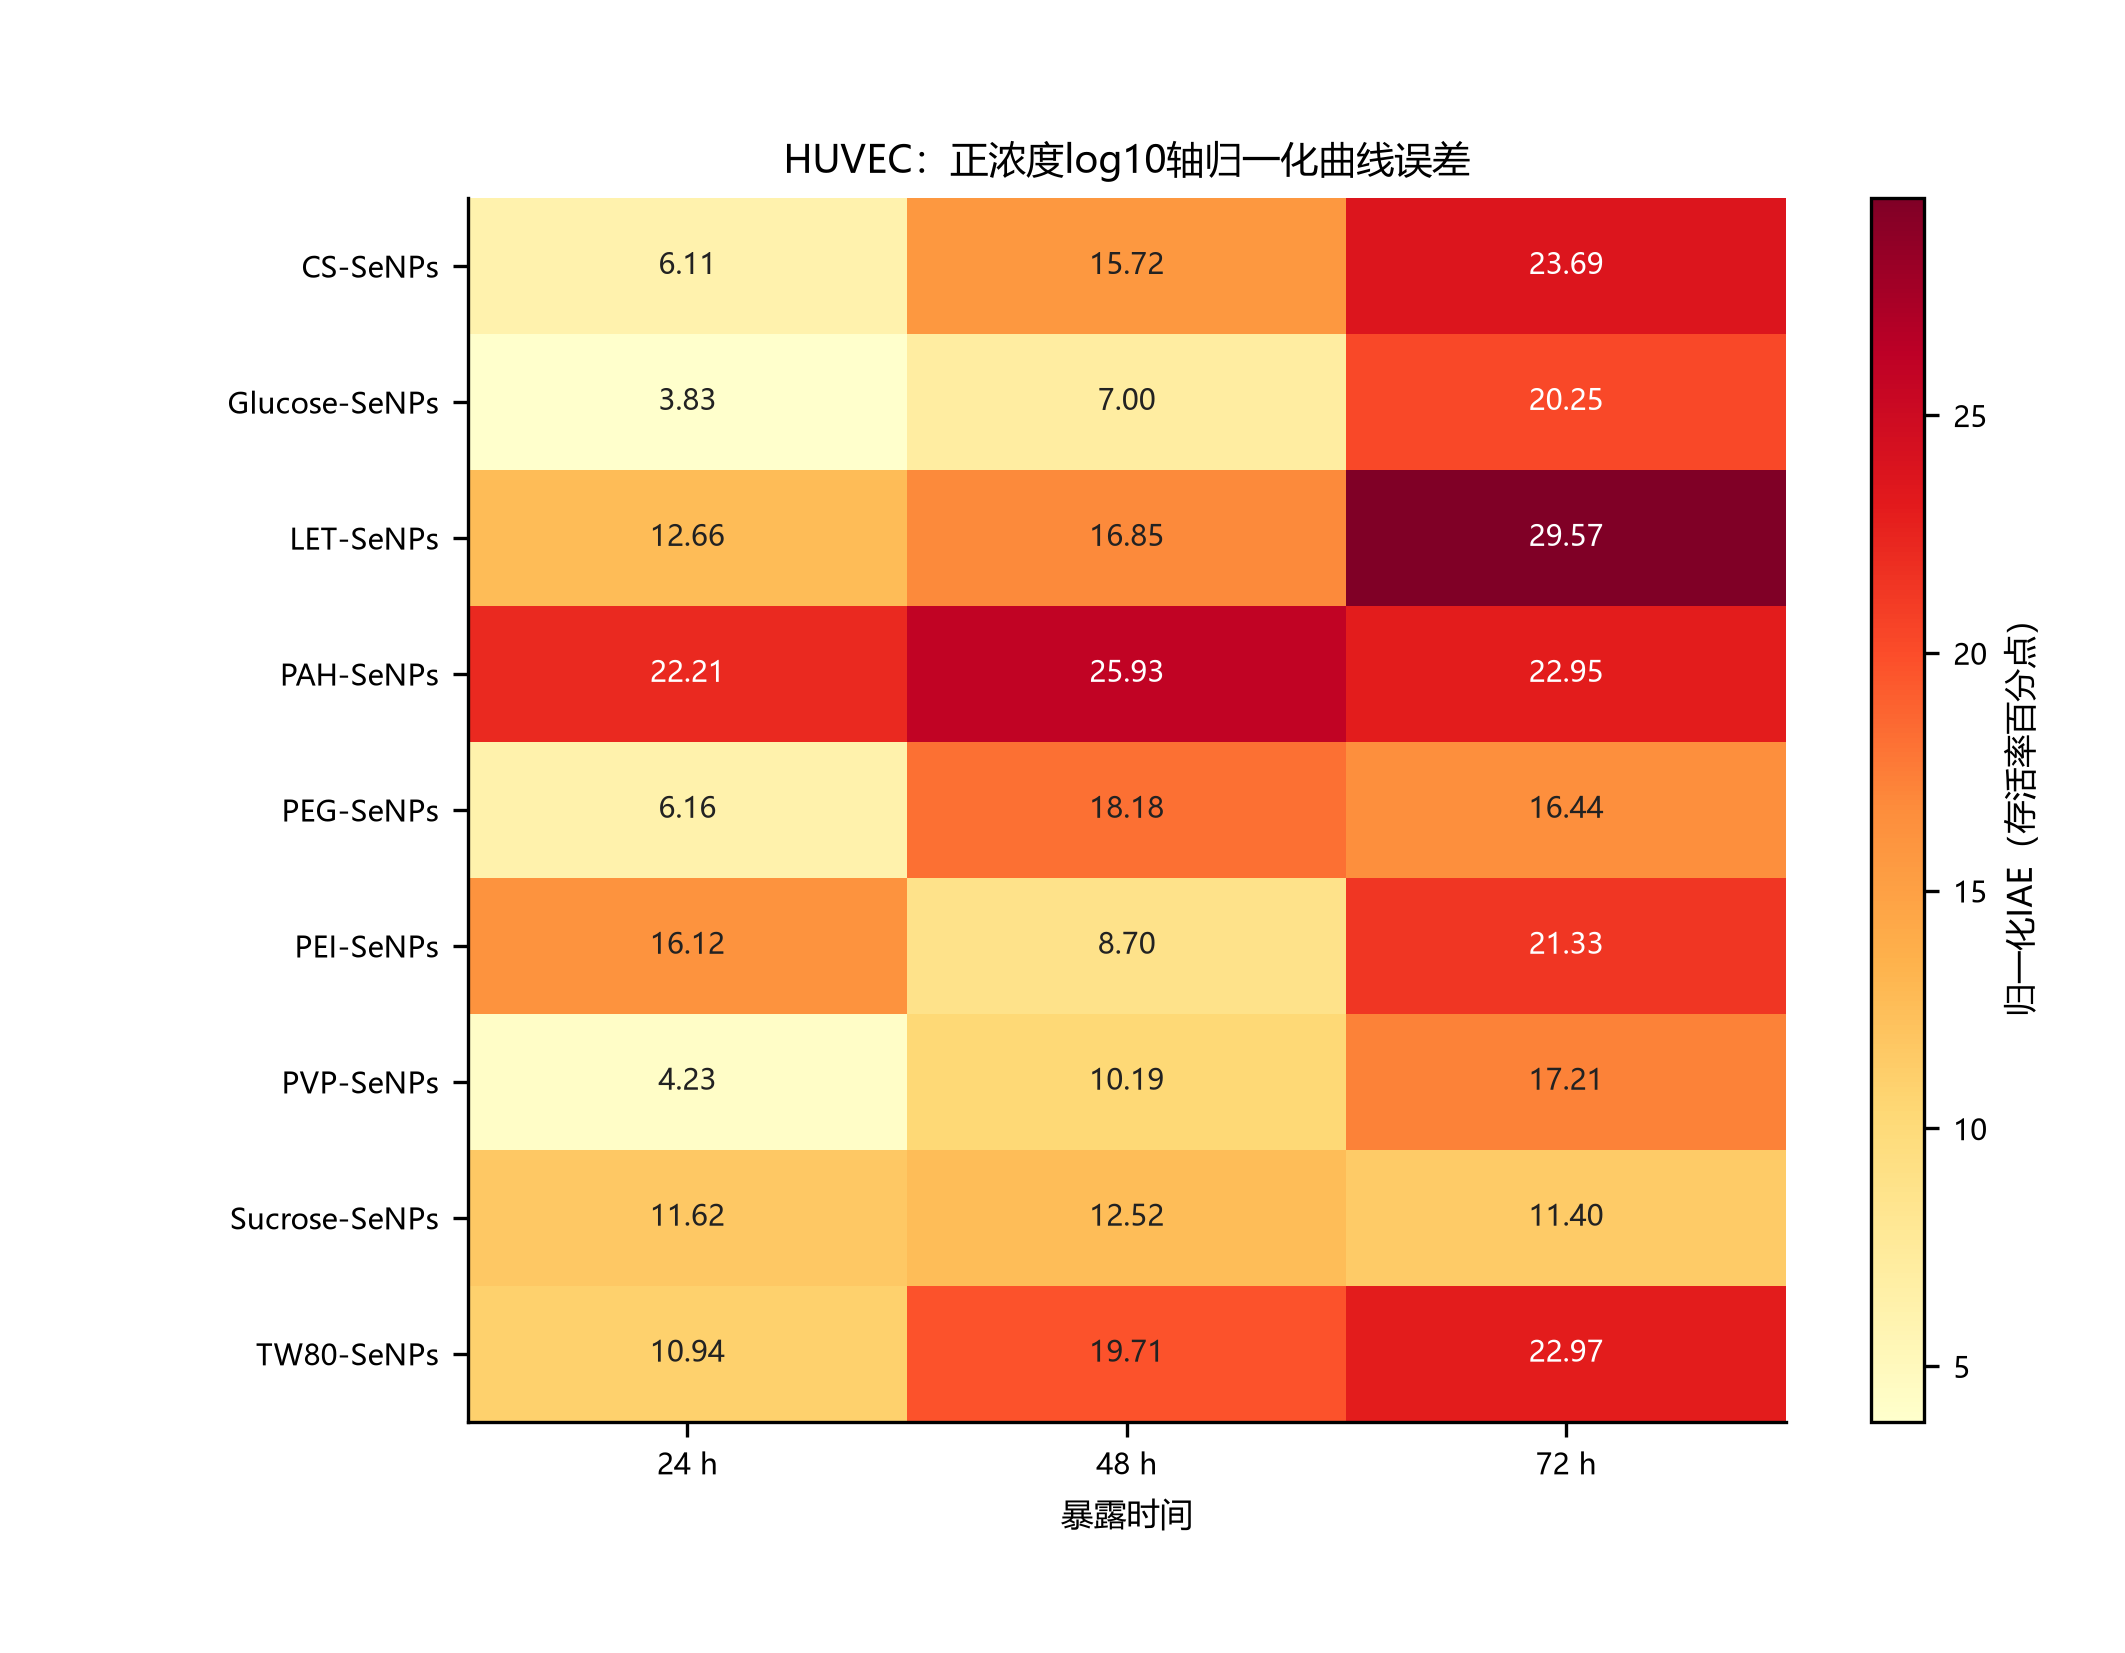
\includegraphics[width=\linewidth,height=0.70\textheight,keepaspectratio]{figures/iae-heatmap.png}
\par{\small 内部核验附图 A. 任务 24 的 IAE 热图。暂不纳入正式正文，待核对积分横轴、零浓度处理、积分区间和数值积分方法后再决定。\par}
\label{fig:huvec_internal_iae}
\end{figure}

\begin{figure}[H]
\centering
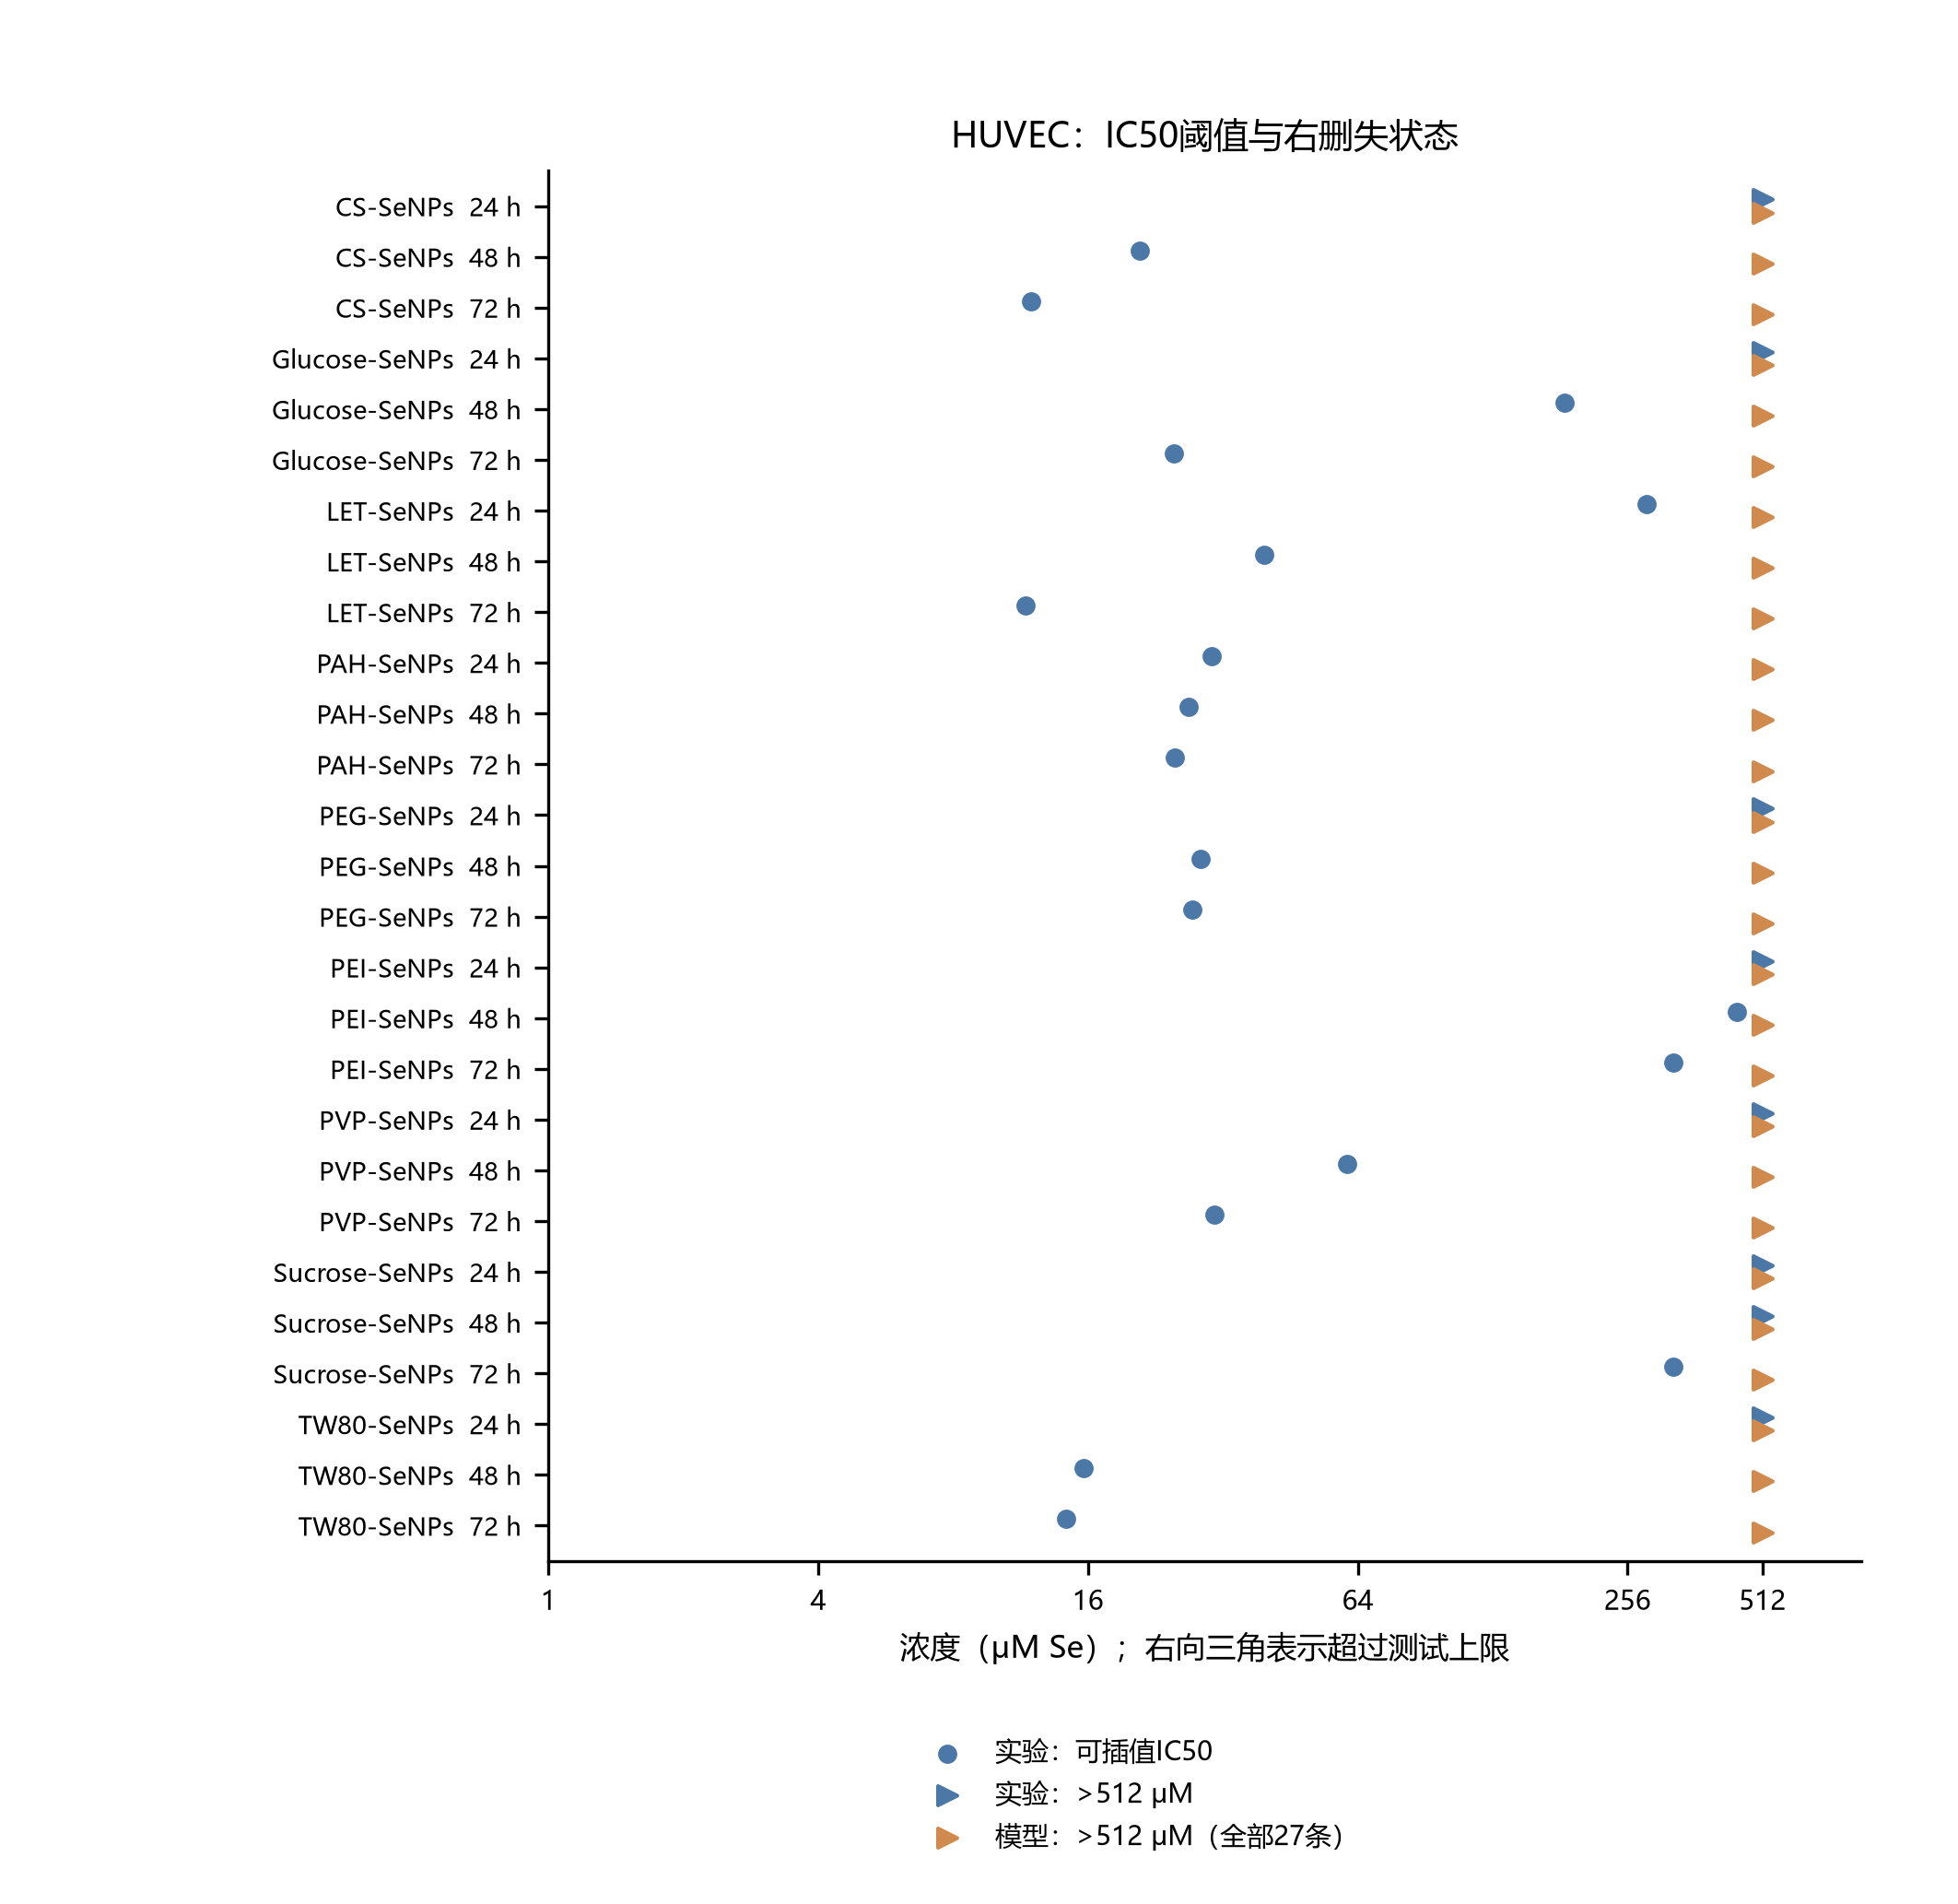
\includegraphics[width=\linewidth,height=0.70\textheight,keepaspectratio]{figures/ic50-pairing.png}
\par{\small 内部核验附图 B. 预测 IC50 与实验 IC50 配对散点图。暂不纳入正式正文。预测曲线未跨越 50\% 存活率阈值，图中有限预测 IC50 及其配对误差目前缺少与曲线一致的可复现依据。\par}
\label{fig:huvec_internal_ic50}
\end{figure}

\subsection*{提交前仍需核验的事项}

核对实验浓度单位、元素硒计量基准及从报告浓度到模型输入浓度的换算方法。

补齐细胞来源、培养条件、检测方法、对照设置、归一化公式、技术重复和独立实验次数。

为 IAE 热图提供可复现的公式和计算脚本，并从预测—实测曲线重新计算。

移除或重新计算任务 26 中无法由预测曲线识别的 pred\_ic50、log\_error 及任何相关 R\textsuperscript{2}。

任务 30 附件已包含 shap\_code\_snippet.py。正式投稿前仍需核对脚本路径与模型、输入文件的归档依赖，并提供可运行的代码存档入口。


\endgroup
\clearpage

%%%%%%%%%%%%%%%%%%%%%%%%%%%%%%%%%%%%%%%%%%%%%%%%%%%%%%%%%%%%%%%%%%%%%
%% If you are using classical BibTeX rather than biblatex,
%% remove the \printbibliography[title={参考文献}] and uncomment the \bibliography one
%%%%%%%%%%%%%%%%%%%%%%%%%%%%%%%%%%%%%%%%%%%%%%%%%%%%%%%%%%%%%%%%%%%%%
\printbibliography
%\bibliography{acs-template.bib}

\newpage

\rule{0.05in}{1.75in}%
\begin{minipage}[b][1.75in]{3.25in}
  \sffamily
  \frenchspacing

  Some journals require a graphical entry for the Table of Contents. This
  should be laid out ``print ready'' so that the sizing of the text is correct.

  The space available depends on the journal: J. Am. Chem. Soc. allows 3.25 in
  by 1.75 in and requires sanserif text. Some journals want different sizes:
  you can easily adjust here.
  
  The two rules either side of the content are there to help judge the height
  of your material: they may be deleted once not required.
  
\end{minipage}%
\rule{0.05in}{1.75in}

\end{document}
